\documentclass[table]{beamer}
\usepackage[utf8]{inputenc}
\usepackage{xcolor}
\usepackage{tcolorbox}
\usepackage{adjustbox}
\usepackage{multicol}
\usepackage{multirow}
\usepackage{eurosym}
\usepackage{amsmath}
\usepackage{ragged2e}
\usepackage[scaled]{helvet}
\usepackage{tikz}
\usepackage{eurosym}
\usetikzlibrary{spy,shapes,arrows,positioning,decorations.pathreplacing}

\tikzset{hide on/.code={\only<#1>{\color{white}}}}
\definecolor{dark_green}{rgb}{0.0, 0.5, 0.0}

\pgfdeclarelayer{bg}    % declare background layer
\pgfsetlayers{bg,main}  % set the order of the layers (main is the standard layer)

\apptocmd{\frame}{}{\justifying}{}

\definecolor{iscal_color}{HTML}{641242} % ISCAL

\setbeamertemplate{footline}{
	\hspace{0.05\textwidth}
	\raisebox{3ex}{\insertshortauthor{}}\hfill
	\raisebox{3ex}{\insertframenumber{}/\inserttotalframenumber} \hfill
	{
\includegraphics[height=0.08\textheight]{../visual material/logo.png}}
	\hspace{0.05\textwidth}
}

\tikzset{
  invisible/.style={opacity=0},
  visible on/.style={alt={#1{}{invisible}}},
  alt/.code args={<#1>#2#3}{%
    \alt<#1>{\pgfkeysalso{#2}}{\pgfkeysalso{#3}} % \pgfkeysalso doesn't change the path
  },
}

\title{Microeconomia}
\subtitle{Capitulo 2 : Teoria do Consumidor}
\author[]{}
\institute[ISCAL]{
\includegraphics[height=0.10\textheight]{../visual material/logo_eng_full.png}}
\date{Primavera 2020/2021}

\setbeamertemplate{navigation symbols}{}

\setbeamercolor{title}{fg = iscal_color}
\setbeamercolor{subtitle}{fg = iscal_color}
\setbeamercolor{frametitle}{fg = white, bg = iscal_color}

\hypersetup{linkcolor=iscal_color, colorlinks=true}

\AtBeginSection{\frame{\sectionpage}}
\renewcommand{\sectionname}{Parte}

\begin{document}

{
\setbeamertemplate{footline}{}
\begin{frame}
	\maketitle
\end{frame}
}

\begin{frame}{Conte\'udos}
  \tableofcontents
\end{frame}

\section{Restri\c c\~ao Or\c camental e Curvas de Indiferen\c ca}
\begin{frame}
	\frametitle{Linguagem}
		\begin{tcolorbox}[colback=blue!5,colframe=blue!40!black,title=Cabaz de Bens]
		\'E composto por quantidades de v\'arios bens. Quando se comparam cabazes, os bens s\~ao os mesmos, mas as quantidades de cada um variam...
	\end{tcolorbox}\pause

	Admitamos dois bens: laranjas ($y$) e bolachas de chocolate ($x$).... ($3,2$) \'e um cabaz composto por por 3 bolachas e 2 laranjas. Gr\'aficamente \'e um ponto do espa\c co ($x,y$)
\end{frame}

\begin{frame}
	\begin{center}
		\begin{tikzpicture}
			\draw[->] (-0.1,0) -- (4.1,0) node[below right] {$x$ bolachas};
			\draw[->] (0,-0.1) -- (0,4.1) node[above left] {$y$ laranjas};

			\draw[dashed] (3,0) node[below]{3} -- (3,2) node[blue,circle,fill,inner sep=2pt]{} -- (0,2) node[left]{2};
		\end{tikzpicture}
	\end{center}
\end{frame}

\begin{frame}
	\frametitle{Conjunto das possibilidades de Consumo}

	\begin{itemize}
		\item \'E o conjunto de todos os cabazes que podem ser adquiridos com um dado or\c camento.
		\item O conjunto de cabazes cuja despesa esgota o or\c camento designa-se ``Restri\c c\~ao Or\c camental''
	\end{itemize}

\end{frame}

\begin{frame}
	\frametitle{Problema do Consumidor}
	De entre os cabazes dispon\'iveis no Espa\c co das Possibilidades de Consumo, encontrar a escolha \'optima, dadas as vari\'aveis ex\'ogenas:\pause

	\vspace{0.2cm}

	\begin{itemize}
		\item Or\c camento ($W$)\pause
		\item Pre\c cos de mercado ($p_x,p_y$)\pause
	\end{itemize}
	\vspace{0.4cm}

	O consumidor ir\'a portanto, decidir o valor para as vari\'aveis end\'ogena, $X$ e $Y$, as suas vari\'aveis de decis\~ao!
\end{frame}

\begin{frame}
	\frametitle{Restri\c c\~ao Or\c camental}
	$$X p_x + Y p_y = W$$
	\euro 10 para gastar em bolachas e laranjas. Cada laranja custa 10 c\^entimos, cada bolacha custa 25 c\^entimos
	
	
	A restri\c c\~ao or\c camental ser\'a... \pause

	$$0.25 X + 0.1 Y = 10$$

\end{frame}

\begin{frame}
	\frametitle{Restri\c c\~ao Or\c camental}

	\begin{center}
		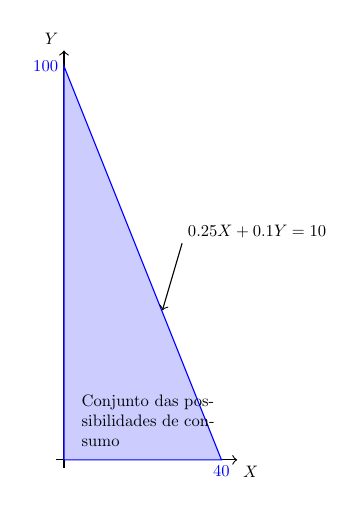
\begin{tikzpicture}[
				every node/.style={scale=0.6},
			]

			\draw[->] (-0.1,0) -- (2.2,0)node[below right]{$X$};
			\draw[->] (0,-0.1) -- (0,5.2)node[above left]{$Y$};

			\draw[blue,fill=blue!20] (0,0) -- (0,5) node[left]{$100$} -- (2,0) node[below]{$40$} -- (0,0);
			
			\draw[->] (1.5,2.75)node[above right]{$0.25X+0.1Y=10$} -- (1.25,1.9);
			\draw (0.15,0.1) node[above right, text width = 0.25\textwidth]{Conjunto das possibilidades de consumo};

		\end{tikzpicture}
	\end{center}
	A Restri\c c\~ao Or\c camental tamb\'em pode ser descrita, neste gr\'afico como $Y = 100 - 2.5X$
\end{frame}

\begin{frame}
	\frametitle{Restri\c c\~ao Or\c camental- Altera\c c\~ao do pre\c co}

	\begin{center}
		\def\w{5}
		\def\dw{1.5}
		\def\px{3}
		\def\py{3.5}
		\def\pxx{4}
		\def\pyy{2.5}
		\begin{tikzpicture}[
				scale = 1.5,
				every node/.style={scale=1},
				declare function = {bc1(\x) = (\w/\py) - (\px/\py)*\x;},
				declare function = {bc2(\x) = (\w/\py) - (\pxx/\py)*\x;},
				declare function = {bc3(\x) = (\w/\pyy) - (\px/\pyy)*\x;}
			]

			\draw[->] (-0.1,0) -- ({\w/2},0)node[below right]{$X$};
			\draw[->] (0,-0.1) -- (0,{\w/2})node[above left]{$Y$};
			
			\only<1>{
				\draw[] (0,{bc1(0)}) node[left] {$\frac{W}{p_Y}$} -- ({\w/\px},{bc1(\w/\px)}) node[below] {$\frac{W}{p_X}$};
				\draw[->] (1,{bc1(1)}) -- (1.5,{bc1(1)+0.55}) node[right]{$Xp_x+Yp_y=W$};
			}

			\only<2>{
				\draw[dashed,gray] (0,{bc1(0)}) node[left] {$\frac{W}{p_Y}$} -- ({\w/\px},{bc1(\w/\px)}) node[below] {$\frac{W}{p_X}$};
				\draw[] (0,{bc2(0)}) node[left] {$\frac{W}{p_Y}$} -- ({\w/\pxx},{bc2(\w/\pxx)}) node[below] {$\frac{W}{\hat{p}_X}$};
				\draw[->] (1,{bc2(1)}) -- (1.5,{bc1(1)+0.55}) node[above right]{Aumento de $p_x$ a $\hat{p}_x$};
			}

			\only<3>{
				\draw[] (0,{bc1(0)}) node[left] {$\frac{W}{p_Y}$} -- ({\w/\px},{bc1(\w/\px)}) node[below] {$\frac{W}{p_X}$};
				\draw[->] (1,{bc1(1)}) -- (1.5,{bc1(1)+0.55}) node[right]{$Xp_x+Yp_y=W$};
			}

			\only<4>{
				\draw[dashed,gray] (0,{bc1(0)}) node[left] {$\frac{W}{p_Y}$} -- ({\w/\px},{bc1(\w/\px)}) node[below] {$\frac{W}{p_X}$};
				\draw[] (0,{bc3(0)}) node[left] {$\frac{W}{\hat{p}_Y}$} -- ({\w/\px},{bc3(\w/\px)}) node[below] {$\frac{W}{p_X}$};
				\draw[->] (1,{bc3(1)}) -- (1.5,{bc3(1)+0.55}) node[above right]{Diminui\c c\~ao de $p_y$ a $\hat{p}_y$};
			}

			\onslide<5->{
				\draw[] (0,{bc1(0)}) node[left] {$\frac{W}{p_Y}$} -- ({\w/\px},{bc1(\w/\px)}) node[below] {$\frac{W}{p_X}$};
			}

			\only<6>{
				\draw[red,domain=0:((\w-\dw)/\px),variable=\x] plot (\x,{bc1(\x)-(\dw/\py)});
				\draw[red] (1.5,{bc1(1)+0.55}) node[above right]{Diminui\c c\~ao de $W$};
			}

			\only<7>{
				\draw[red,domain=0:((\w+\dw)/\px),variable=\x] plot (\x,{bc1(\x)+(\dw/\py)});
				\draw[red] (1.5,{bc1(1)+0.55}) node[above right]{Aumento de $W$};
			}			

		\end{tikzpicture}
	\end{center}
\end{frame}

\begin{frame}
	\frametitle{Declive da Restri\c c\~ao Or\c camental}
	\begin{align*}
		X P_x + Y p_y = W \quad \Leftrightarrow \quad Y = {\color{red}\frac{W}{p_y}} - {\color{blue}\frac{p_x}{p_y}}X
	\end{align*}

	\begin{itemize}
		\item $\frac{W}{p_y}$: {\color{red}Ordenada na Origem}
		\item $-\frac{p_x}{p_y}$: {\color{blue}Declive}
	\end{itemize}

	$$0.25X + 0.1Y = 10 \quad \Leftrightarrow \quad Y = {\color{red}100} - {\color{blue}2.5} X$$
\end{frame}


\begin{frame}
	\frametitle{Escolha \'optima do consumidor}
	Do conjunto das possibilidades de consumo, escolher o cabaz \'optimo ($x,y$) em fun\c c\~ao de:\pause
	\vspace{0.2cm}
	\begin{itemize}
		\item Vari\'aveis ex\'ogenas (pre\c cos, rendimento)
		\item Prefer\^encias...
			\begin{itemize}
				\item Axiom\'atica de prefer\^encias
			\end{itemize}
	\end{itemize}
\end{frame}

\begin{frame}
	\frametitle{Axiom\'atica de Prefer\^encias}
	\begin{itemize}
		\item \textbf{Desejabilidade} ou \textbf{N\~ao Saciedade}: Consumir mais, \'e melhor
	\end{itemize}

	Ent\~ao, por exemplo, o consumidor vai preferir o cabaz $A=(25,30)$ ao cabaz $B=(20,20)$ simplesmente porque o cabaz $A$ cont\'em mais quantidade (para ambos bens) do que o cabaz $B$.

\end{frame}

\begin{frame}
	\frametitle{Desejabilidade}
	\begin{center}
		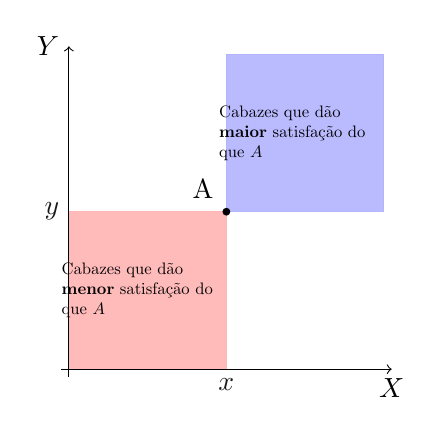
\begin{tikzpicture}
			\draw[fill,red!30,opacity=0.9] (0,0) -- (0,2) node[black,left] {$y$} -- (2,2) -- (2,0) node[black,below]{$x$} -- (0,0);
			\draw[fill,blue!30,opacity=0.9] (2,2) -- (4,2) -- (4,4) -- (2,4) -- (2,2);

			\draw[->] (-0.1,0) -- (4.1,0) node[below]{$X$};
			\draw[->] (0,-0.1) -- (0,4.1) node[left]{$Y$};

			\draw(2,2) node[circle,fill,inner sep=1pt,label = above left:A]{};
			\draw(1,1) node[text width = 0.3\textwidth, scale = 0.6] {Cabazes que d\~ao \textbf{menor} satisfa\c c\~ao do que $A$};
			\draw(3,3) node[text width = 0.3\textwidth, scale = 0.6] {Cabazes que d\~ao \textbf{maior} satisfa\c c\~ao do que $A$};
		\end{tikzpicture}
	\end{center}

\end{frame}

\begin{frame}
	\frametitle{Axiom\'atica de Prefer\^encias}
	E se um cabaz cont\'em mais de um bem e menos do outro?! Qual o preferido? (20,30) ou (30,20)?!?
	\vspace{0.2cm}
	\begin{itemize}
		\item<1-> \'E preciso saber quais s\~ao os cabazes indiferentes entre si...
		\item<2-> Quantas laranjas est\'a o consumidor disposto a abdicar, para ter mais uma bolacha de chocolate e ficar indiferente?
		\begin{itemize}
			\item<3-> A resposta n\~ao depende do que pode comprar dadas as suas possibilidades de consmo, mas apenas das prefer\^encias.
		\end{itemize}
	\end{itemize}

\end{frame}

\begin{frame}
	\frametitle{Curva de Indiferen\c ca}
	\begin{tcolorbox}[title=Curva de indiferen\c ca]
		Conjunto dos cabazes indiferentes entre si!
	\end{tcolorbox}

	\begin{itemize}
		\item<2-> Devido \`a hip\'otese de desejabilidade, os cabazes indiferentes entre si n\~ao podem conter mais quantidade de ambos os bens, nem podem conter menos quantidade de ambos os bens: t\^em de conter sempre mais de um e menos do outro.
		\item<3-> No espa\c co $XY$, a curva de indiferen\c ca tem de ter inclina\c c\~ao negativa!
	\end{itemize}

\end{frame}

\begin{frame}
	\frametitle{Curva de Indiferen\c ca}
	\begin{center}
		\def\a{1/2}
		\begin{tikzpicture}[
			scale = 1,
			declare function = {i(\x) = (1/(\x^\a))^(1/(1-\a));},
		]

		\draw[->] (0,-0.1) -- (0,5.1) node[left]{$Y$};
		\draw[->] (-0.1,0) -- (5.1,0) node[below]{$X$};

		\draw[domain=1:4,variable=\x] plot (\x,{i(\x)});

		\draw[dotted] (0,{i(1.5)}) node[left] {35} -- (1.5,{i(1.5)}) node[circle,fill,inner sep=1pt,label = above right:A]{} -- (1.5,0)node[below] {15};
		\draw[dotted] (0,{i(2)}) node[left] {20} -- (2,{i(2)}) node[circle,fill,inner sep=1pt,label = above right:B]{} -- (2,0)node[below] {20};
		\draw[dotted] (0,{i(3)}) node[left] {15} -- (3,{i(3)}) node[circle,fill,inner sep=1pt,label = above right:C]{} -- (3,0)node[below] {30};

		\draw(1,{i(1)}) node[above]{U};

		\draw(4,4) node[right,text width = 0.5\textwidth, scale = 0.7] {Se $U$ for uma curva de indiferen\c ca, ent\~ao $A$, $B$ e $C$ s\~ao cabazes indiferentes entre si...};

		\end{tikzpicture}
	\end{center}
\end{frame}
\section{Taxa marginal de substitui\c c\~ao e Fun\c c\~ao de utilidade}
\begin{frame}
	\frametitle{Taxa Marginal de Substitui\c c\~ao}
	\begin{itemize}
		\item<1-> \'E a taxa \`a qual o consumidor est\'a disposto a trocar um bem pelo outro e ficar indiferente.
		\item<2-> Define-se como a quantidade do bem $Y$ de que est\'a disposto a prescindir, para ter mais uma unidade do bem $X$ e ficar indiferente.
	\end{itemize}
\end{frame}

\begin{frame}
	\frametitle{Taxa Marginal de Subsitui\c c\~ao}
	\begin{center}
		\def\a{1/2}
		\begin{tikzpicture}[
			scale = 1,
			declare function = {i(\x) = (1/(\x^\a))^(1/(1-\a));},
			declare function = {di(\x) = -(\a/(1-\a))*(1/(\x^(1/(1-\a))));},
			declare function = {tang(\x) = i(1.5) - (i(3)-i(1.5)) + ((i(3)-i(1.5))/(3-1.5)) * \x;},
			declare function = {tg(\x) = tang(\x) - 0.35;}
		]

		\draw[->] (0,-0.1) -- (0,5.1) node[left]{$Y$};
		\draw[->] (-0.1,0) -- (5.1,0) node[below]{$X$};

		\draw(3.5,5.1) node[above] {$\Delta Y/\Delta X$};

		\draw[domain=1:4,variable=\x] plot (\x,{i(\x)});

		\draw[dotted] (0,{i(1.5)}) node[left] {35} -- (1.5,{i(1.5)}) node[circle,fill,inner sep=1pt,label = above right:A]{} -- (1.5,0)node[below] {15};
		\draw[dotted] (0,{i(3)}) node[left] {15} -- (3,{i(3)}) node[circle,fill,inner sep=1pt,label = above right:C]{} -- (3,0)node[below] {30};

		\only<1>{
			\draw[dotted] (0,{i(2)}) node[left] {20} -- (2,{i(2)}) node[circle,fill,inner sep=1pt,label = above right:B]{} -- (2,0)node[below] {20};
			\draw(4,4) node[right,text width = 0.5\textwidth, scale = 0.9] {De A a B: $TMS = -3 = \frac{-15}{5}$};
			\draw(4,3.5) node[right,text width = 0.5\textwidth, scale = 0.9] {De B a C: $TMS = -0.5 = \frac{-5}{10}$};
		}

		\onslide<2->{
			\draw(3.5,4) node[right,text width = 0.6\textwidth, scale = 0.8] {De A a C: $TMS = \frac{\Delta Y}{\Delta X} = -1.3 = \frac{-20}{15}$};
			\draw[blue,thick,domain=0:(-(2*i(1.5)-i(3))*(3-1.5)/(i(3)-i(1.5))),variable=\x] plot (\x,{tang(\x)});
		}
		
		\onslide<3->{
			\draw[blue,thick,->] (1.5,{tang(1.5)}) -- (1.5,{tang(3)}) node [midway, left,scale=0.6] {$\Delta Y$};
		}
		\onslide<4->{
			\draw[blue,thick,->] (1.5,{tang(3)}) -- (3,{tang(3)}) node [midway, below,scale=0.6] {$\Delta X$};
		}
		
		\onslide<5->{
			\draw[red,thick,dashed,domain=1:3,variable=\x] plot (\x,{tg(\x)}); 
		}

		\onslide<6->{
			\draw[fill,blue!20] (3,{i(3)}) node[black,scale=0.8,above left] {$\alpha\ \ $} -- (2.5,{tang(3)}) -- (2.6,{tang(2.6)});
			\draw(3.5,3.5) node[right,text width = 0.6\textwidth, scale = 0.8] {$TMS=tg(\alpha)$};
		}

		\onslide<7->{
			\draw[] (3.5,3) node[below right,rectangle,draw=red!50,scale=0.8,text width=0.6\textwidth] {TMS \'e o declive da Curva de Indiferen\c ca num ponto entre $A$ e $C$ (Teorema de Lagrange)};
		}

		\end{tikzpicture}
	\end{center}
\end{frame}

\begin{frame}
	\frametitle{Taxa Marginal de Substitui\c c\~ao}
	Ao longo da curva de indiferen\c ca apresentada (convexa), a TMS \'e decrescente em valor absoluto:
	\vspace{0.2cm}
	\begin{itemize}
		\item<2-> Admitimos que o consumidor valoriza mais o bem de que disp\~oe em menor quantidade
		\item<3-> Quanto maior a quantidade de um bem de que o consumidor disp\~oe, menor o valor que atribui a uma unidade adicional, porque fica mais perto do ponto de saciedade, onde o consumo adicional deixa de ser desej\'avel!
	\end{itemize}
\end{frame}

\begin{frame}
	\frametitle{Axiom\'atica de Prefer\^encias (cont.)}
	\begin{enumerate}
		\item<2->Desejabilidade $\Rightarrow$ as curvas de indiferen\c ca t\^em inclina\c c\~ao negativa!
		\item<3->As prefer\^encias s\~ao completas: dados dois cabazes, o consumidor sabe sempre dizer qual a rela\c c\~ao de prefer\^encias entre eles $\Rightarrow$ todos os cabazes pertencem a uma curva de indiferen\c ca!
		\begin{itemize}
			\item<4-> Quanto mais alta for a curva onde se localiza um cabaz, maior a satisfa\c c\~ao que resulta do consumo desse cabaz (desejabilidade...)
		\end{itemize}
	\end{enumerate}
\end{frame}

\begin{frame}
	\frametitle{Curvas de Indiferen\c ca ``bem comportadas''}
	\begin{center}
		\def\a{1/2}
		\begin{tikzpicture}[
			scale = 1,
			declare function = {i(\x,\u) = (\u/(\x^\a))^(1/(1-\a));}
		]

		\draw[->] (0,-0.1) -- (0,5.1) node[left]{$Y$};
		\draw[->] (-0.1,0) -- (5.1,0) node[below]{$X$};

		\draw[samples=100,domain=0.9:5,variable=\x] plot (\x,{i(\x,1)});

		\draw (2,{i(2,1)}) node[circle,fill,inner sep=1pt,label = above right:A]{};
		\draw (1.1,{i(1.1,1)}) node[circle,fill,inner sep=1pt,label = above right:B]{};

		\draw (2.2,{i(2.2,2)}) node[circle,fill,inner sep=1pt,label = above right:C]{};
		\draw (3,{i(3,2)}) node[circle,fill,inner sep=1pt,label = above right:D]{};

		\draw (2.6,{i(2.6,3)}) node[circle,fill,inner sep=1pt,label = above right:E]{};
		\draw (3.2,{i(3.2,3)}) node[circle,fill,inner sep=1pt,label = above right:F]{};

		\draw (1.2,{i(1.2,0.6)}) node[circle,fill,inner sep=1pt,label = above right:G]{};
		
		\onslide<2->{
			\draw [samples=100,blue,domain=1.8:5,variable=\x] plot (\x,{i(\x,2)});
			\draw [samples=100,blue,domain=2.5:5,smooth,variable=\x] plot (\x,{i(\x,3)});
			\draw [samples=100,red,domain=0.6:5,variable=\x] plot (\x,{i(\x,0.6)});
		}

		\only<3-4>{
			\draw[] (4.5,5) node[above right,scale=0.7] {$\sim$ Significa ``indiferente a''};
			\draw[] (4.5,4.5) node[above right,scale=0.7] {$\succ$ Significa ``preferido a''};

		}

		\only<4>{
			\draw[] (4.5,4) node[above right, scale=0.7] {$E\sim F\succ C\sim D \succ B \sim A \succ G$};
			\draw[->,thick,green] (1,1) -- (4,4) node [green!80!black,below right,scale=0.8] {Sentido de aumento da satisfa\c c\~ao};
		}
		\end{tikzpicture}
	\end{center}
\end{frame}

\begin{frame}
	\frametitle{Axiom\'atica de Prefer\^encias (cont.)}
	\begin{enumerate}
		\item<1-> Desejabilidade
		\item<2-> As prefer\^encias s\~ao completas
		\item<3-> As prefer\^encias s\~ao transitivas:
	\end{enumerate}
	\onslide<3->{Se:
	\begin{center}
		A \'e preferido a B\\
		B \'e preferido a C\\
		Ent\~ao A \'e preferido a C!
	\end{center}
	}
\end{frame}

\begin{frame}
	\frametitle{As curvas de Indiferen\c ca n\~ao se podem cruzar}
	\begin{columns}
		\begin{column}{0.47\textwidth}
			\begin{center}
				\def\a{1/2}
				\def\inter{1.365}
				\begin{tikzpicture}[
						scale = 0.7,
						every node/.style = {scale = 0.7},
						declare function = {i(\x,\u) = (\u/(\x^\a))^(1/(1-\a));}
					]

					\draw[->] (0,-0.1) -- (0,5.1) node[left]{$Y$};
					\draw[->] (-0.1,0) -- (5.1,0) node[below]{$X$};

					\draw[domain=0.9:5,variable=\x] plot (\x,{i(\x,1)});
					\draw[domain=0.5:4.5,variable=\x] plot (\x,{i(\x+0.5,1)+1});

					\draw (2,{i(2,1)}) node[circle,fill,inner sep=1.5pt,label = above right:A]{};
					\draw (1.1,{i(1.1,1)}) node[circle,fill,inner sep=1.5pt,label = above right:B]{};

					\draw (\inter,{i(\inter,1)}) node[circle,fill,inner sep=1.5pt,label = above right:C]{};
					\draw (2.2,{i(2.7,1)+1}) node[circle,fill,inner sep=1.5pt,label=above right:D]{};
					
			\end{tikzpicture}
			\end{center}
		\end{column}
		\begin{column}{0.47\textwidth}
			\begin{itemize}
				\item Estas curvas de indiferen\c ca n\~ao refleitem prefer\^encias transitivas.
				\item<2-> $D\succ A$
				\item<3-> Pero $D\sim C$,
				\item<4-> E $C\sim A$!!!
			\end{itemize}
		\end{column}
	\end{columns}
\end{frame}

\begin{frame}
	\frametitle{Racionalidade}
	\begin{itemize}
		\item<1-> Em contexto de desejabilidade (n\~ao saciedade), as prefer\^encias dizem-se racionais, se forem completas e transitivas.
		\item<2-> Outras hip\'oteses necess\'arias na Teoria do Consumidor:
		\begin{itemize}
			\item<3-> Informa\c c\~ao completa
			\item<4-> Continuidade do espa\c co or\c camental
			\item<5-> Independ\^encia das escolhas entre consumidores
		\end{itemize}
	\end{itemize}
\end{frame}


\begin{frame}
	\frametitle{Fun\c c\~ao Utilidade}
	A fun\c c\~ao de utilidade \'e uma representa\c c\~ao num\'erica da rela\c c\~ao de prefer\^encia, que transforma cabazes de consumo num valor (utilidade) e \'e tal que dados dois cabazes $A$ e $B$:
	\begin{align*}
		U(A) &> U(B) \quad \Leftrightarrow \quad \text{A \'e preferido a B}\\
		U(A) &= U(B) \quad \Leftrightarrow \quad \text{A \'e indiferente a B}
	\end{align*}
\end{frame}


\begin{frame}
	\frametitle{Fun\c c\~ao Utilidade}
	A fun\c c\~ao de utilidade \'e apenas uma \textbf{\underline{rela\c c\~ao ordinal}}, resultando numa ordena\c c\~ao de cabazes, atribuindo um valor maior aos cabazes preferidos. \textbf{\underline{Esse valor, por si s\'o, n\~ao tem significado cardinal.!}}\pause

	\vspace{0.2cm}

	\underline{Consequ\^encia:} h\'a muitas fun\c c\~oes utilidade que expressam as mesmas prefer\^encias, basta que preservem a ordena\c c\~ao dos cabazes...
\end{frame}

\begin{frame}
	\frametitle{Fun\c c\~ao Utilidade}
	Ex. $A(20,20)$ \'e preferido a $B(10,10)$. Esta rela\c c\~ao pode ser descrita por qualquer uma das fun\c c\~oes seguintes:
	\begin{align*}
		U(x,y) &= x^{0.5}y^{0.5}\\
		U(x,y) &= 10x^{0.5}y^{0.5}\\
		U(x,y) &= 0.5(ln(x)+ln(y))\\
		U(x,y) &= 223.2(ln(x)+ln(y))
	\end{align*}
\end{frame}


\begin{frame}
	\frametitle{Fun\c c\~ao Utilidade}
	Se uma fun\c c\~ao utilidade $U(x,y)$ representar uma ordem de prefer\^encias, qualquer curva de indeferen\c ca \'e constitu\'ida por todos os cabazes que est\~ao associados \`a mesma utilidade:
	\begin{align*}
		\forall(x,y)&:U(x,y)=\overline{U}\\
		&\text{ou}\\
		\forall(x,y)&:\Delta U = 0
	\end{align*}
\end{frame}

\begin{frame}
	\frametitle{Escolha \'Optima}
	\'E o ponto de escolha tal que o consumidor atinge o m\'aximo de utilidade poss\'ivel (localiza-se na curva de indiferen\c ca o mais alta poss\'ivel), dado que n\~ao pode ultrapassar o or\c camento dispon\'ivel para consumo.
\end{frame}

\begin{frame}
	\frametitle{Escolha do consumidor}
	\begin{center}
		\def\a{0.5}
		\def\u{1.55}
		\def\d{0.5}
		\def\w{10}
		\def\px{3}
		\def\py{3.5}
		\begin{tikzpicture}[
			scale = 1,
			every node/.style={scale = 1},
			declare function = {ic(\x,\u) = ((\u)/(\x^\a))^(1/(1-\a));},
			declare function = {bc(\x,\w) = \w/\py - (\px/\py)*\x;}
			]

			\draw[->] (-0.1,0) -- (5.1,0)node[below right] {$X$};
			\draw[->] (0,-0.1) -- (0,5.1)node[above left] {$Y$};

			\draw[] (4,4) node[right,scale=0.6] {$A^{*}(P,W):Max_{x,y} U(x,y)\wedge Xp_x+Yp_y=W$};

			\onslide<2->{\draw[samples=100,blue,domain=0:(\w/\px),variable=\x] plot (\x,{bc(\x,\w)});}
			\onslide<3-4>{\draw[samples=100,red,domain=1:5,variable=\x] plot (\x,{ic(\x,\u+\d)});}
			\only<4>{\draw[samples=100,red,domain=.3:5,variable=\x] plot (\x,{ic(\x,\u-\d)});}
			\onslide<5->{
				\draw[samples=100,red,domain=.6:5,variable=\x] plot (\x,{ic(\x,\u)});
				\draw(1.65,{ic(1.65,\u)}) node[red,circle,fill,inner sep=1.5pt]{};
				\draw[dashed](1.65,0) node[below]{$x^*$} -- (1.65,{ic(1.65,\u)}) -- (0,{ic(1.65,\u)}) node [left]{$y^*$};
			}
 
		\end{tikzpicture}
	\end{center}
\end{frame}
\section{Formaliza\c c\~ao Anal\'itica do Problema do Consumidor}
\begin{frame}
	\frametitle{Escolha do consumidor}
	\begin{center}
		\def\a{0.5}
		\def\u{1.55}
		\def\d{0.5}
		\def\w{10}
		\def\px{3}
		\def\py{3.5}
		\begin{tikzpicture}[
			scale = 1,
			every node/.style={scale = 1},
			declare function = {ic(\x,\u) = ((\u)/(\x^\a))^(1/(1-\a));},
			declare function = {bc(\x,\w) = \w/\py - (\px/\py)*\x;}
			]

			\draw[->] (-0.1,0) -- (5.1,0)node[below right] {$X$};
			\draw[->] (0,-0.1) -- (0,5.1)node[above left] {$Y$};

			\draw[] (4,4) node[right,scale=0.6] {$A^{*}(P,W):Max_{x,y} U(x,y)\wedge Xp_x+Yp_y=W$};

			\draw[samples=100,blue,domain=0:(\w/\px),variable=\x] plot (\x,{bc(\x,\w)});
			
			\draw[samples=100,red,domain=.6:5,variable=\x] plot (\x,{ic(\x,\u)});
			\draw(1.65,{ic(1.65,\u)}) node[red,circle,fill,inner sep=1.5pt]{};
			\draw[dashed](1.65,0) node[below]{$x^*$} -- (1.65,{ic(1.65,\u)}) -- (0,{ic(1.65,\u)}) node [left]{$y^*$};
		 
		\end{tikzpicture}
	\end{center}
\end{frame}

\begin{frame}
	\frametitle{Observa\c c\~ao}
	No cabaz de escolha \'optima o declive da restri\c c\~ao or\c camental \'e igual ao declive da curva de indiferen\c ca \pause

	\vspace{0.2cm}

	Declive da restri\c c\~ao or\c camental \'e $-\frac{p_x}{p_y}$\pause

	\vspace{0.2cm}

	Qual o declive da curva de indiferen\c ca? \'E a TMS... No \'optimo, ambos os declives t\^em de ser iguais!

\end{frame}

\begin{frame}
	\frametitle{Leis de Gossen}
	\begin{tcolorbox}[title=2\textsuperscript{a} Lei]
		No cabaz \'optimo, $$\left|TMS\right|=\frac{p_x}{p_y}$$
	\end{tcolorbox}
	TMS \'e o declive da curva de indiferen\c ca num ponto, mas tamb\'em tem uma rela\c c\~ao com a utilidade... precisamos tamb\'em da 1\textsuperscript{a} Lei!.
\end{frame}

\begin{frame}
	\frametitle{Utilidade Total - Utilidade Marginal}

	\begin{itemize}
		\item<1-> \textbf{Utilidade total:} n\'ivel de satisfa\c c\~ao que o consumidor retira ao consumir uma certa quantidade de um bem - medida pela fun\c c\~ao de utilidade...
		\item<2-> \textbf{Utilidade marginal:} utilidade fornecida pelo consumo de uma unidade adicional desse bem
			- medida pela varia\c c\~ao m\'edia da fun\c c\~ao utilidade, quando uma vari\'avel $X$ se altera, \emph{c\ae teris paribus}, ou seja, a derivada:  $$\frac{\Delta U}{\Delta X} = Umg_{x}=U'_{x}$$
	\end{itemize}
\end{frame}

\begin{frame}
	\frametitle{Utilidade Total vs Umg}
	\begin{columns}
		\begin{column}{0.47\textwidth}
			\begin{center}
				\begin{tikzpicture}[
					scale = 0.8,
					every node/.style = {scale = 0.8},
					declare function = {f(\x)=2*\x^(1/4);}
					]

					\draw[->] (0,-0.1) -- (0,4.1) node[left]{$U$};
					\draw[->] (-0.1,0) -- (4.1,0) node[below]{$X$};

					\onslide<2->{\draw[dashed] (0.5,0)node[below]{$x_0$} -- (0.5,{f(0.5)}) -- (0,{f(0.5)})node[left]{$U(x_0)$};}
					\onslide<3->{\draw[dashed] (2.5,0)node[below]{$x_1$} -- (2.5,{f(2.5)}) -- (0,{f(2.5)})node[left]{$U(x_1)$};}


					\draw[samples=200,domain=0:4,variable=\x] plot (\x,{f(\x)});

				\end{tikzpicture}
			\end{center}
		\end{column}
		\begin{column}{0.47\textwidth}
			\begin{center}
				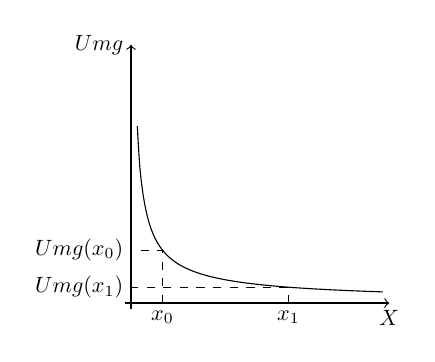
\begin{tikzpicture}[
					scale = 0.8,
					every node/.style = {scale = 0.8},
					declare function = {f(\x)=(1/2)*\x^(-3/4);}
					]

					\draw[->] (0,-0.1) -- (0,4.1) node[left]{$Umg$};
					\draw[->] (-0.1,0) -- (4.1,0) node[below]{$X$};

					\onslide<4->{\draw[dashed] (0.5,0)node[below]{$x_0$} -- (0.5,{f(0.5)}) -- (0,{f(0.5)})node[left]{$Umg(x_0)$};}
					\onslide<5->{\draw[dashed] (2.5,0)node[below]{$x_1$} -- (2.5,{f(2.5)}) -- (0,{f(2.5)})node[left]{$Umg(x_1)$};}

					\draw[samples=200,domain=0.1:4,variable=\x] plot (\x,{f(\x)});
				\end{tikzpicture}
			\end{center}
		\end{column}
	\end{columns}

	\vspace{0.2cm}

	\onslide<6->{Estamos a aproximar o ponto de saciedade! $\rightarrow$ O ponto em que o consumo de um adicional n\~ao aumenta a satisfa\c c\~ao, ou seja o ponto em que $Umg=0$}
\end{frame}

\begin{frame}
	\frametitle{Leis de Gossen}
	\begin{itemize}
		\item \textbf{1\textsuperscript{a} Lei de Gossen:} uma unidade adicional de um bem tem uma utilidade adicional cada vez menor \`a medida que o consumo vai aumentando - a utilidade marginal \'e descrescente!
		\item<2->\textbf{3\textsuperscript{a} Lei de Gossen:} \'e a da escassez, que vem o valor econ\'omico
	\end{itemize}
\end{frame}

\begin{frame}
	\frametitle{Utilidade Marginal}
	A utilidade marginal influencia directamente a disponibilidade a pagar por mais uma unidade de um bem:
	\begin{itemize}
		\item<2->Quanto mais se consome de um bem, menor a utilidade marginal de mais uma unidade, ou
		\item<3-> Menor o valor que o consumidor lhe atribui, portanto, menor a sua disponibilidade a pagar...
	\end{itemize}
	\onslide<3->{\textbf{Pre\c co de reserva:} m\'aximo que o consumidor est\'a disposto a pagar por uma unidade adicional do bem.}
\end{frame}

\begin{frame}
	\frametitle{TMS e Utilidade Marginal}
	Uma Curva de Indiferen\c ca cont\'em todos os cabazes indiferentes a um cabaz $A$, ou seja, todos os cabazes dessa curva t\^em uma tuilidade igual a $U(A)$!

	\vspace{0.2cm}

	Ao longo da curva de indiferen\c ca, alterar $X$ ou $Y$ n\~ao pode alterar $U(A)$, caso contr\'ario n\~ao se estaria ainda na mesma curva...
\end{frame}

\begin{frame}
	\frametitle{TMS e Umg}
	$A\rightarrow C$ redu\c c\~ao de $Y$ \emph{c\ae teris paribus}\\
	$C\rightarrow B$ aumento de $X$ \emph{c\ae teris paribus}
	\begin{center}
		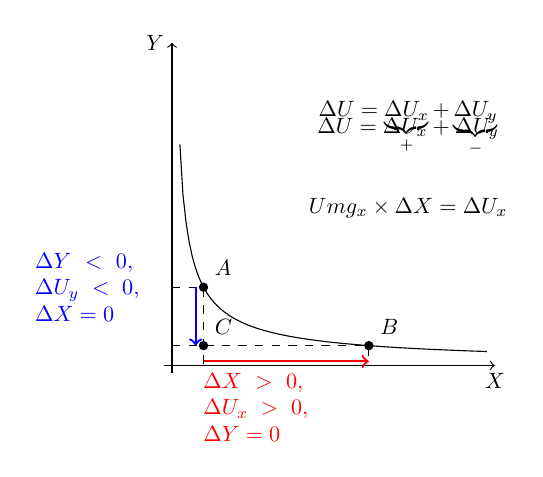
\begin{tikzpicture}[
			scale = 1,
			every node/.style = {scale = 0.8},
			declare function = {f(\x)=(1/2)*\x^(-3/4);}
		]

			\draw[->] (0,-0.1) -- (0,4.1) node[left]{$Y$};
			\draw[->] (-0.1,0) -- (4.1,0) node[below]{$X$};

			\draw[samples=100,domain=0.1:4,variable=\x] plot (\x,{f(\x)});

			\onslide<2->{
				\draw[dashed] (0,{f(0.4)}) -- (0.4,{f(0.4)}) node[circle,fill,inner sep=1.5pt,label=above right:$A$]{} -- (0.4,0);
				\draw[dashed] (0,{f(2.5)}) -- (2.5,{f(2.5)}) node[circle,fill,inner sep=1.5pt,label=above right:$B$]{} -- (2.5,0);
			}
			\onslide<3->{
				\draw (0.4,{f(2.5)}) node[circle,fill,inner sep=1.5pt,label=above right:$C$] {};
			}

			\onslide<4->{
				\draw[->,thick,blue] (0.3,{f(0.4)}) -- (0.3,{f(2.5)});
				\draw (0.3,{f(0.4)}) node[blue,left,text width = 0.2\textwidth] {$\Delta Y<0$, $\Delta U_y < 0$, $\Delta X = 0$};
			}
			
			\onslide<6->{
				\draw[->,thick,red] (0.4,{f(2.5)-0.2}) -- (2.5,{f(2.5)-0.2});
				\draw (0.3,0) node[red,below right,text width = 0.2\textwidth] {$\Delta X>0$, $\Delta U_x > 0$, $\Delta Y = 0$};
			}

			\onslide<7>{
				\draw(3,3) node[]{$\Delta U = \Delta U_x + \Delta U_y$};
			}

			\onslide<8>{
				\draw(3,3) node[]{$\Delta U = \underbrace{\Delta U_x}_{+} + \underbrace{\Delta U_y}_{-}$};
				\draw(3,2) node[]{$Umg_x\times\Delta X = \Delta U_x$};
			}

		\end{tikzpicture}
	\end{center}
\end{frame}

\begin{frame}
	\frametitle{TMS e Utilidade Marginal}
	Ao longo da Curva de Indiferen\c ca, $\Delta U = 0$

	Se $X$ ou $Y$ alterarem a sua quantidade, a altera\c c\~ao em $U$ \'e:
	\begin{align*}
		\onslide<2->{\Delta U &= Umg_x \times \Delta X + Umg_y \times \Delta Y}\\
		\onslide<3->{\Delta U = 0\quad &\Leftrightarrow\quad Umg_x \Delta X = -Umg_y \Delta Y \\
		&\text{ou,}}\\
		\onslide<4->{\frac{\Delta Y}{\Delta X} &= -\frac{Umg_x}{Umg_y}=TMS}
	\end{align*}
\end{frame}

\begin{frame}
	\frametitle{TMS e 1\textsuperscript{a} Lei de Gossen}
	\begin{itemize}
		\item Verific\'amos que $|TMS|$ \'e decrescente \`a medida que $X$ aumenta e $Y$ diminui
		\item<2-> Se $\frac{Umg_x}{Umg_y}=|TMS|$ e dada a 1\textsuperscript{a} Lei de gossen:
	\end{itemize}

	\onslide<2->{
		\begin{align*}
			\left.
			\begin{array}{c}
				\downarrow Y \quad\Rightarrow\quad \uparrow Umg_y\\
				\uparrow X \quad\Rightarrow\quad \downarrow Umg_x\\
			\end{array}\right\}\Rightarrow \quad\downarrow \frac{Umg_x}{Umg_y} = \downarrow TMS
		\end{align*}
	}
\end{frame}

\begin{frame}
	\frametitle{TMS e 1\textsuperscript{a} Lei de Gossen}
	O consumidor $A$ valoriza o bem $Y$ muito mais do que o consumidor $B$

	\begin{columns}
		\begin{column}{0.47\textwidth}
			\begin{center}
				\begin{tikzpicture}[
					scale = 0.8,
					every node/.style = {scale = 0.8},
					declare function = {f(\x)=(1/2)*\x^(-3/4);}
					]

					\draw[->] (0,-0.1) -- (0,4.1) node[left]{$Y$};
					\draw[->] (-0.1,0) -- (4.1,0) node[below]{$X$};

					\onslide<2->{\draw[dashed] (0.5,0)node[below]{$x_0$} -- (0.5,{f(0.5)}) -- (0,{f(0.5)})node[left]{$y_0$};}
					\onslide<3->{\draw[dashed] (2.5,0)node[below]{$x_1$} -- (2.5,{f(2.5)}) -- (0,{f(2.5)})node[left]{$y_1$};}

					\draw[samples=200,domain=0.1:4,variable=\x] plot (\x,{f(\x)});
				\end{tikzpicture}
				Consumidor $A$
			\end{center}
		\end{column}
		\begin{column}{0.47\textwidth}
			\begin{center}
				\begin{tikzpicture}[
					scale = 0.8,
					every node/.style = {scale = 0.8},
					declare function = {f(\x)=(1)*\x^(-1);}
					]

					\draw[->] (0,-0.1) -- (0,4.1) node[left]{$Y$};
					\draw[->] (-0.1,0) -- (4.1,0) node[below]{$X$};

					\onslide<2->{\draw[dashed] (0.5,0)node[below]{$x_0$} -- (0.5,{f(0.5)}) -- (0,{f(0.5)})node[left]{$y_0$};}
					\onslide<3->{\draw[dashed] (2.5,0)node[below]{$x_1$} -- (2.5,{f(2.5)}) -- (0,{f(2.5)})node[left]{$y_1$};}

					\draw[samples=200,domain=0.3:4,variable=\x] plot (\x,{f(\x)});
				\end{tikzpicture}
				Consumidor $B$
			\end{center}
		\end{column}
	\end{columns}
\end{frame}
\section{Procura Individual}
\begin{frame}
	\frametitle{Escolha do consumidor}

	\begin{itemize}
		\item Um consumidor racional disp\~oe de um presente de \euro 160 para gastar em cal\c cas e em camisas para renovar o seu vestu\'ario.
		\item Uma camisa (bem $x$) custa \euro 20 e um par de cal\c cas (bem $y$) custa \euro 30.
		\item As prefer\^encias podem ser descritas pela fun\c c\~ao $U(x,y)=xy^3$
	\end{itemize}

	\begin{enumerate}
		\item Qual a escolha racional, que maximiza $U$?
		\item Qual a equa\c c\~ao da curva de indiferen\c ca no \'optimo?
	\end{enumerate}

\end{frame}

\begin{frame}
	\frametitle{Escolha do consumidor}

	\onslide<1->{\[U(x,y)=xy^3\]}\\

	\onslide<2->{\[Umg_x = \onslide<3->{y^3}\quad\wedge\quad Umg_y=\onslide<3->{3xy^2}\]}\\

	\onslide<3->{\[\frac{Umg_x}{Umg_y}=\frac{y^3}{3xy^2}=\frac{y}{3x}\]}\\

	\onslide<4->{\[|TMS|=\frac{y}{3x}\]}

\end{frame}

\begin{frame}
	\frametitle{Escolha do consumidor}
	\onslide<1->{
		Restri\c c\~ao Or\c camental: \[30y+20x=160\]
	}

	\onslide<2->{
		De onde podemos encontrar: \[\frac{p_x}{p_y}=\frac{20}{30}=\frac{2}{3}\]
	}

	\onslide<3->{
		E segundo a \onslide<4->{2\textsuperscript{a} lei de Gossen} temos que no \'otimo: \[|TMS|=\frac{p_x}{p_y}\]
	}

	\onslide<5->{
		\[\Rightarrow\quad \frac{y^*}{3x^*} = \frac{2}{3} \quad \Leftrightarrow \quad y^* = 2x^*\]
	}

\end{frame}

\begin{frame}
	\frametitle{Escolha do consumidor}

	Para cumprir com a Restri\c c\~ao Or\c camental, \'e for\c coso que:
	
	\onslide<1->{
		\[30y+20x=160\]
	}

	\onslide<2->{
		\[30\times \overbrace{2x^*}^{y^*=2x^*} + 20x^* = 160\]
	}

	\onslide<3->{
		\[60x^*+20x^*=160 \quad \Leftrightarrow \quad 80x^* = 160\]
	}

	\onslide<4->{
		Ent\~ao $x^*=\frac{160}{80}=2$, e porque $y^*=2x^*$ temos que $y^*=2\times 2 = 4$.

		Assim $U(2,4)=2\times 4^3 = 2\times 64=128$.
	}

\end{frame}

\begin{frame}
	\frametitle{Escolha do consumidor}

	Como no \'optimo $U=128$, ent\~ao podemos encontrar a curva de indifer\^en\c ca:

	\onslide<2->{
		\[U = 128 = xy^3\]
		\[y^3 = \frac{128}{x}\]
		\[y = \left(\frac{128}{x}\right)^{\frac{1}{3}} = \sqrt[3]{\frac{128}{x}}\]
	}

\end{frame}


\begin{frame}
	\frametitle{Escolha do consumidor}
	\begin{center}
		\begin{tikzpicture}[
			scale = 0.8,
			every node/.style={scale = 0.8},
			declare function = {ic(\x) = (128/\x)^(1/3);},
			declare function = {bc(\x) = (16/3) - (2/3)*\x;}
			]

			\draw[->] (-0.1,0) -- (9.1,0)node[below right] {$X$};
			\draw[->] (0,-0.1) -- (0,6.1)node[above left] {$Y$};

			\draw[samples=100,blue,domain=0:(16/2),variable=\x] plot (\x,{bc(\x)});
			
			\draw[samples=100,red,domain=.6:5,variable=\x] plot (\x,{ic(\x)});
			\draw(2,{ic(2)}) node[red,circle,fill,inner sep=1.5pt]{};
			\draw[dashed](2,0) node[below]{$x^*=2$} -- (2,{ic(2)}) -- (0,{ic(2)}) node [left]{$y^*=4$};
		 
		\end{tikzpicture}
	\end{center}
\end{frame}

\begin{frame}
	\frametitle{Custo-Benef\'icio}
	2\textsuperscript{a} Lei de Gossen e escolha \'optima \[\frac{Umg_x}{Umg_y}=\frac{p_x}{p_y}\]

	Consumir mais uma unidade tem um custo marginal \(\frac{p_x}{p_y}\) e um benef\'icio marginal \(\frac{Umg_x}{Umg_y}=|TMS|\)...

	a 2\textsuperscript{a} Lei de Gossen tem impl\'icita a an\'alise custo benef\'icio...
\end{frame}

\begin{frame}
	\frametitle{Dedu\c c\~ao da Procura Individual}
	Iremos considerar uma altera\c c\~ao no pre\c co de mercado de um dos bens e estudar o que acontece aos pontos de escolha \'optima...

	{\color{red}Intui\c c\~ao: se um pre\c co subir, tudo o resto constante, o que acontece \`a quantidade consumida? E porqu\^e?}
\end{frame}

\begin{frame}
	\frametitle{Dedu\c c\~ao da Procura Individual}
	\begin{center}
			Redu\c c\~ao do pre\c co de $x$: $p_x^0>p_x^1>p_x^2$
			\def\rho{0.5}
			\def\ww{15}
			\def\pyy{3}
			\begin{tikzpicture}[
				scale = 0.8,
				every node/.style={scale = 0.8},
				declare function={
					x(\w,\px,\py) = (\w*(\px^(1/(\rho-1))))/(\px^(\rho/(\rho-1))+\py^(\rho/(\rho-1)));
					y(\w,\px,\py) = (\w*(\py^(1/(\rho-1))))/(\px^(\rho/(\rho-1))+\py^(\rho/(\rho-1)));
					u(\x,\y) = (\x^\rho+\y^\rho)^(1/\rho);
					ic2(\x,\px,\py) = (u(x(\ww,\px,\py),y(\ww,\px,\py))^\rho-\x^\rho)^(1/\rho);
					bc2(\x,\px,\py) = \ww/\py - (\px/\py)*\x;
				}
				]

				\draw[->] (-0.1,0) -- (9.1,0)node[below right] {$X$};
				\draw[->] (0,-0.1) -- (0,6.1)node[above left] {$Y$};


				\onslide<2->{
					\draw[samples=100,blue,domain=0:(\ww/4),variable=\x] plot (\x,{bc2(\x,4,\pyy)});
					\draw({\ww/4},0) node[circle,fill,inner sep=1.5pt,label=below :\(\frac{W}{p_x^0}\)]{};
					\draw(0,{\ww/\pyy}) node[circle,fill,inner sep=1.5pt,label=left :\(\frac{W}{p_y}\)]{};
					\draw[samples=100,red,domain=.55:7,variable=\x] plot (\x,{ic2(\x,4,\pyy)});
					\draw({x(\ww,4,\pyy)},{y(\ww,4,\pyy)}) node[red,circle,fill,inner sep=1.5pt]{};
				}

				\onslide<3->{
					\draw[samples=100,blue,domain=0:(\ww/3),variable=\x] plot (\x,{bc2(\x,3,\pyy)});
					\draw({\ww/3},0) node[circle,fill,inner sep=1.5pt,label=below :\(\frac{W}{p_x^1}\)]{};
					\draw(0,{\ww/\pyy}) node[circle,fill,inner sep=1.5pt,label=left :\(\frac{W}{p_y}\)]{};
					\draw[samples=100,red,domain=.70:7,variable=\x] plot (\x,{ic2(\x,3,\pyy)});
					\draw({x(\ww,3,\pyy)},{y(\ww,3,\pyy)}) node[red,circle,fill,inner sep=1.5pt]{};
				}

				\onslide<4->{
					\draw[samples=100,blue,domain=0:(\ww/2),variable=\x] plot (\x,{bc2(\x,2,\pyy)});
					\draw({\ww/2},0) node[circle,fill,inner sep=1.5pt,label=below :\(\frac{W}{p_x^2}\)]{};
					\draw(0,{\ww/\pyy}) node[circle,fill,inner sep=1.5pt,label=left :\(\frac{W}{p_y}\)]{};
					\draw[samples=100,red,domain=1.2:7,variable=\x] plot (\x,{ic2(\x,2,\pyy)});
					\draw({x(\ww,2,\pyy)},{y(\ww,2,\pyy)}) node[red,circle,fill,inner sep=1.5pt]{};
				}

				\onslide<5->{
					\draw[thick,blue] plot[smooth, tension=0.7] coordinates{(1,3) ({x(\ww,4,\pyy)},{y(\ww,4,\pyy)}) ({x(\ww,3,\pyy)},{y(\ww,3,\pyy)}) ({x(\ww,2,\pyy)},{y(\ww,2,\pyy)}) (7,1)} node[right]{Via Pre\c co Consumo};
				}

			\end{tikzpicture}
		\end{center}
\end{frame}

\begin{frame}
	\frametitle{Dedu\c c\~ao da Procura Individual - Curva Pre\c co Consumo}
	\begin{center}
			Redu\c c\~ao do pre\c co de $x$: $p_x^0>p_x^1>p_x^2$

			\def\rho{0.5}
			\def\ww{15}
			\def\pyy{3}
			\begin{tikzpicture}[
				scale = 0.8,
				every node/.style={scale = 0.8},
				declare function={
					x(\w,\px,\py) = (\w*(\px^(1/(\rho-1))))/(\px^(\rho/(\rho-1))+\py^(\rho/(\rho-1)));
					y(\w,\px,\py) = (\w*(\py^(1/(\rho-1))))/(\px^(\rho/(\rho-1))+\py^(\rho/(\rho-1)));
					u(\x,\y) = (\x^\rho+\y^\rho)^(1/\rho);
					ic2(\x,\px,\py) = (u(x(\ww,\px,\py),y(\ww,\px,\py))^\rho-\x^\rho)^(1/\rho);
					bc2(\x,\px,\py) = \ww/\py - (\px/\py)*\x;
				}
				]

				\draw[->] (-0.1,0) -- (9.1,0)node[below right] {$X$};
				\draw[->] (0,-0.1) -- (0,6.1)node[above left] {$Y$};

				\draw({x(\ww,4,\pyy)},{y(\ww,4,\pyy)}) node[red,circle,fill,inner sep=1.5pt,label=above:\(p_x^0\)]{};
				\draw({x(\ww,3,\pyy)},{y(\ww,3,\pyy)}) node[red,circle,fill,inner sep=1.5pt,label=above:\(p_x^1\)]{};
				\draw({x(\ww,2,\pyy)},{y(\ww,2,\pyy)}) node[red,circle,fill,inner sep=1.5pt,label=above:\(p_x^2\)]{};

				\draw[thick,blue] plot[smooth, tension=0.7] coordinates{(1,3) ({x(\ww,4,\pyy)},{y(\ww,4,\pyy)}) ({x(\ww,3,\pyy)},{y(\ww,3,\pyy)}) ({x(\ww,2,\pyy)},{y(\ww,2,\pyy)}) (7,1)};

			\end{tikzpicture}
		\end{center}
\end{frame}

\begin{frame}
	\frametitle{Dedu\c c\~ao da Procura Individual}
	N\~ao h\'a raz\~ao para assumir que a Curva de Pre\c co Consumo tem uma forma est\'andar (crescente, descrescente, etc). O que vai determinar o que se passa perante um cambio no pre\c co de $x$ s\~ao as prefer\^encias. A Curva Pre\c co Consumo tamb\'em \'e conhecida como Offer Curve.\pause

	O que sabemos \'e que n\~ao pode ir para acima de\pause $\frac{W}{p_y}$.
\end{frame}

\begin{frame}
	\frametitle{Dedu\c c\~ao da Procura Individual}
	\begin{center}

			\def\rho{0.5}
			\def\ww{15}
			\def\pyy{3}
			\begin{tikzpicture}[
				scale = 0.4,
				every node/.style={scale = 0.5},
				declare function={
					x(\w,\px,\py) = (\w*(\px^(1/(\rho-1))))/(\px^(\rho/(\rho-1))+\py^(\rho/(\rho-1)));
					y(\w,\px,\py) = (\w*(\py^(1/(\rho-1))))/(\px^(\rho/(\rho-1))+\py^(\rho/(\rho-1)));
					u(\x,\y) = (\x^\rho+\y^\rho)^(1/\rho);
					ic2(\x,\px,\py) = (u(x(\ww,\px,\py),y(\ww,\px,\py))^\rho-\x^\rho)^(1/\rho);
					bc2(\x,\px,\py) = \ww/\py - (\px/\py)*\x;
				}
				]

				\draw[->] (-0.1,0) -- (9.1,0)node[below right] {$X$};
				\draw[->] (0,-0.1) -- (0,6.1)node[above left] {$Y$};

				\draw({x(\ww,4,\pyy)},{y(\ww,4,\pyy)}) node[red,circle,fill,inner sep=1.5pt,label=above:\(p_x^0\)]{};
				\draw({x(\ww,3,\pyy)},{y(\ww,3,\pyy)}) node[red,circle,fill,inner sep=1.5pt,label=above:\(p_x^1\)]{};
				\draw({x(\ww,2,\pyy)},{y(\ww,2,\pyy)}) node[red,circle,fill,inner sep=1.5pt,label=above:\(p_x^2\)]{};

				\draw[blue] plot[smooth, tension=0.7] coordinates{(1,3.5) ({x(\ww,4,\pyy)},{y(\ww,4,\pyy)}) ({x(\ww,3,\pyy)},{y(\ww,3,\pyy)}) ({x(\ww,2,\pyy)},{y(\ww,2,\pyy)}) (6,1)};

				\onslide<2->{
					\draw[->] (-0.1,-8) -- (9.1,-8)node[below right] {$X$};
					\draw[->] (0,-8.1) -- (0,-1.9)node[above left] {$p_x$};

					\draw[dotted] ({x(\ww,4,\pyy)},{y(\ww,4,\pyy)}) -- ({x(\ww,4,\pyy)},-8);
					\draw[dotted] ({x(\ww,3,\pyy)},{y(\ww,3,\pyy)}) -- ({x(\ww,3,\pyy)},-8);
					\draw[dotted] ({x(\ww,2,\pyy)},{y(\ww,2,\pyy)}) -- ({x(\ww,2,\pyy)},-8);
				}

				\onslide<3->{
					\draw[dotted] (0,{4-8})node[left]{\(p_x^0\)} -- ({x(\ww,4,\pyy)},{4-8});
					\draw[dotted] (0,{3-8})node[left]{\(p_x^1\)} -- ({x(\ww,3,\pyy)},{3-8});
					\draw[dotted] (0,{2-8})node[left]{\(p_x^2\)} -- ({x(\ww,2,\pyy)},{2-8});
			 	}

			 	\onslide<4->{
			 		\draw[thick,green] plot[smooth,tension=0.4] coordinates{(1,-3.5) ({x(\ww,4,\pyy)},{4-8}) ({x(\ww,3,\pyy)},{3-8}) ({x(\ww,2,\pyy)},{2-8}) (6,-6.5)} node[black,below right]{\parbox[l]{4cm}{Curva de Procura Individual pelo bem \(x\)}};
			 	}

			\end{tikzpicture}
		\end{center}
\end{frame}

\begin{frame}
	\frametitle{Curva da Procura}
	\'E o conjunto dos pares $(Q,P)$ de escolha \'optima, para diferentes pre\c cos, dado um valor fixo para as vari\'aveis ex\'ogenas \`as decis\~oes do consumidor:\pause
	\begin{itemize}
		\item Rendimento dispon\'ivel\pause
		\item Pre\c co dos outros bens\pause
		\item Prefer\^encias e factores que as influenciem
	\end{itemize}
\end{frame}

\begin{frame}
	\frametitle{Lei da Procura}
	Entre a quantidade procurada de um bem e o pre\c co desse mesmo bem, existe uma rela\c c\~ao negativa: 
	\begin{tcolorbox}[colback=iscal_color!10,colframe=iscal_color]
		Se o pre\c co aumenta, a quantidade procurada diminui, \emph{c\ae teris paribus}
	\end{tcolorbox}

	\footnotesize{Aten\c c\~ao: dada a altera\c c\~ao de pre\c co, trata-se de uma altera\c c\~ao da quantidade, ou seja, das inten\c c\~oes de consumo/compra...}
\end{frame}

\begin{frame}
	\frametitle{A Lei da Procura}
	\begin{center}
		\begin{tikzpicture}[
			scale = 1,
			every node/.style={scale = 1},
			declare function = {d1(\x) = 6-1.3*(\x^(0.8));}
		]

		\draw[->] (-0.1,0) -- (6.1,0)node[below right] {$X$};
		\draw[->] (0,-0.1) -- (0,6.1)node[above left] {$p_x$};

		\onslide<2->{
			\draw[blue,thick,domain=0.6:5.4,variable=\x,samples=100] plot (\x,{d1(\x)});
			\draw(5.4,{d1(5.4)}) node[right]{\(D\)};
		}

		\onslide<3->{
			\draw[dashed] (4,0) node[below]{4} -- (4,{d1(4)}) node[circle,fill,inner sep=1.5pt,label=above right:$a$]{} -- (0,{d1(4)}) node[left]{2};
		}

		\onslide<4->{
			\draw(0,{d1(3)}) node[left]{3};
			\draw[thick,red,->](0,{d1(4)}) -- (0,{d1(3)});
		}

		\onslide<5->{
			\draw[dashed] (3,0) node[below]{3} -- (3,{d1(3)}) node[circle,fill,inner sep=1.5pt,label=above right:$b$]{} -- (0,{d1(3)}) node[left]{3};
			\draw[->,thick,red] (4,{d1(4)}) -- (3,{d1(3)});
			\draw[->,thick,red] (4,0) -- (3,0);
		}

		\end{tikzpicture}
	\end{center}
\end{frame}

\begin{frame}
	\frametitle{Curva de Procura}
	Mudan\c cas no \textbf{pre\c co} v\~ao causar movimentos \textbf{ao longo} da curva de procura.

	\vspace{0.4cm}

	\'E importante distinguir entre mudan\c cas na procura, de mudan\c cas na \emph{quantidade procurada}.

	\vspace{0.4cm}

	Quando definimos a procura, temos quantidade procurada para um pre\c co, ou seja a quantidade \'e fun\c c\~ao do pre\c co, $Q_x=f(p_x)$.

	\vspace{0.4cm}

	Assim, no nosso gr\'afico temos ao contr\'ario, ou seja tempos o pre\c co associado \'a um n\'ivel de quantidade procurada, ou seja $P=g(Q_x)$. Esta curva de procura tambem \'e conhecida como \textbf{procura inversa}. Isto \'e, na verdade, a mesma coisa que a procura s\'o que vista desde um ponto de vista diferente.

\end{frame}

\begin{frame}
	\frametitle{Procura}

	Se a altera\c c\~ao de um pre\c co, \emph{caeteris paribus}, leva a uma altera\c c\~ao de um ponto para outro na mesma curva de procura, ent\~ao o que faz alterar a posi\c c\~ao da curva?!?

\end{frame}

\begin{frame}
	\frametitle{Que vari\'aveis afectam a Procura?}
	A quantidade de um bem que os consumidores adquirir depende de:

	\begin{columns}
		\begin{column}{0.65\textwidth}
			\begin{itemize}
				\item \(p =\) pre\c co de adquisi\c c\~ao {\color{red}(-)}
					\begin{itemize}
						\item Na mesma curva, passase para outro ponto
					\end{itemize}
				\item \(p_r =\) pre\c co de bens relacionados no consumo:
					\begin{itemize}
						\item Bens substitutos {\color{red}(+)}
						\item Bens complement\'arios {\color{red}(-)}
					\end{itemize}
				\item \(W=\) rendimento dispon\'ivel para consumo
					\begin{itemize}
						\item Bem normal {\color{red}(+)}
						\item Bem inferior {\color{red}(-)}
					\end{itemize}
				\item Prefer\^encias e factores que as afectem
			\end{itemize}
		\end{column}
		\begin{column}{0.3\textwidth}
			\onslide<2->{
			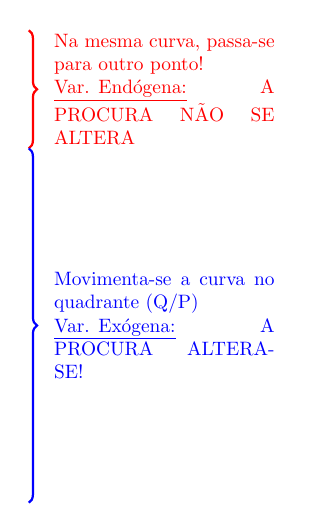
\begin{tikzpicture}[
				scale = 1,
				every node/.style = {scale = 0.7}
				]
				\draw [decorate,decoration={brace,mirror,amplitude=3pt},thick,red] (0,3.5) -- (0,5) node [midway,xshift=70pt] {\parbox{4cm}{Na mesma curva, passa-se para outro ponto!\\ \underline{Var. End\'ogena:} A PROCURA N\~AO SE ALTERA}};
				
				\draw [decorate,decoration={brace,mirror,amplitude=3pt},thick,blue] (0,-1) -- (0,3.5) node [midway,xshift=70pt] {\parbox{4cm}{Movimenta-se a curva no quadrante (Q/P)\\ \underline{Var. Ex\'ogena:} A PROCURA ALTERA-SE!}};
			\end{tikzpicture}
			}
		\end{column}
	\end{columns}

\end{frame}

\begin{frame}
	\frametitle{Classifica\c c\~ao entre bens dada a sua rela\c c\~ao de consumo}
	\begin{itemize}
		\item Bens substitutos
		\begin{itemize}
			\item Altera\c c\~oes no pre\c co de um dos bens implicam varia\c c\~oes no mesmo sentido na procura do outro bem.
			\item Quando o pre\c co de um bem aumenta, a procura do outro bem aumenta
		\end{itemize}
		\item Bens complementares
		\begin{itemize}
			\item Altera\c c\~oes no pre\c co de um dos bens implicam varia\c c\~oes no sentido oposto na procura do outro bem
			\item Quando o pre\c co de um aumenta, a procura do outro diminui.
		\end{itemize}
	\end{itemize}
\end{frame}

\begin{frame}
	\frametitle{Classifica\c c\~ao entre bens dada a sua rela\c c\~ao com o rendimento}
	\begin{itemize}
		\item Bem normal
		\begin{itemize}
			\item A sua procura aumenta quando o rendimento aumenta
			\item Aumentos no rendimento deslocam a curva de procura para a direita
		\end{itemize}
		\item Bem inferior
		\begin{itemize}
			\item Aumentos no rendimento fazem diminuir a sua procura
			\item Aumento no rendimento faz a curva deslocar-se para a esquerda
		\end{itemize}
	\end{itemize}
\end{frame}

\begin{frame}
	\frametitle{Procura}
	\begin{itemize}
		\item \`A rela\c c\~ao funcional entre a quantidade procurada de um bem e todas as vari\'aveis que a infuienciam, chama-se \underline{Fun\c c\~ao Procura}: \[Q_d=f(p,p_r,W,...)\]
		\item A curva de procura obt\'em-se estudando a rela\c c\~ao que existe entre a quantidade procurada, {\color{red}\(Q_D\)}, e o seu pre\c co, {\color{red}\(p\)}, para valores \textbf{dados} das outras vari\'aveis.

		{\small (que n\~ao est\~ao representadas nos eixos, onde se representa o gr\'afico da Procura)}
	\end{itemize}
\end{frame}

\begin{frame}
	\frametitle{Expans\~ao da Procura}
	Que altera\c c\~ao de vari\'aveis ex\'ogenas poderia estar na origem da desloca\c c\~ao da procura?
	\begin{center}
		\begin{tikzpicture}[
			scale = 1,
			every node/.style={scale = 1},
			declare function = {
				d1(\x) = 5.5-1.3*(\x^(0.8));
				d2(\x) = 6.5-1.3*(\x^(0.8));
			}
		]

		\draw[->] (-0.1,0) -- (6.1,0)node[below right] {$X$};
		\draw[->] (0,-0.1) -- (0,6.1)node[above left] {$p_x$};
		\draw[blue,thick,domain=0.6:5.4,variable=\x,samples=100] plot (\x,{d1(\x)}) node[right]{D};
		\draw[dashed] (3,0) node[below]{3} -- (3,{d1(3)}) node[circle,fill,inner sep=1.5pt,label=below left:$b$]{} -- (0,{d1(3)}) node[left]{3};
		
		\onslide<2->{
			\draw[red,thick,domain=0.6:5.4,variable=\x,samples=100] plot (\x,{d2(\x)}) node[right]{\(D'\)};
		}

		\onslide<3-4>{
			\draw[thick,blue,->] (3,{d1(3)}) -- (3,{d2(3)});
		}

		\only<4>{
			\draw[thick,blue,->] (3,{d1(3)}) -- (4.2,{d1(3)});
		}

		\end{tikzpicture}
	\end{center}
\end{frame}

\begin{frame}
	\frametitle{Expans\~ao da Procura}
	Que altera\c c\~ao de vari\'aveis ex\'ogenas poderia estar na origem da desloca\c c\~ao da procura?
	\begin{center}
		\begin{tikzpicture}[
			scale = 1,
			every node/.style={scale = 1},
			declare function = {
				d1(\x) = 5.5-1.3*(\x^(0.8));
				d2(\x) = 6.5-1.3*(\x^(0.8));
			}
		]

		\draw[->] (-0.1,0) -- (6.1,0)node[below right] {$X$};
		\draw[->] (0,-0.1) -- (0,6.1)node[above left] {$p_x$};
		
		\onslide<2->{
			\draw[red,thick,domain=0.6:5.4,variable=\x,samples=100] plot (\x,{d1(\x)}) node[right]{\(D'\)};
			
		}

		\onslide<1->{
			\draw[blue,thick,domain=0.6:5.4,variable=\x,samples=100] plot (\x,{d2(\x)}) node[right]{\(D\)};
			\draw[dashed] (3,0) node[below]{3} -- (3,{d2(3)}) node[circle,fill,inner sep=1.5pt,label=above right:$b$]{} -- (0,{d2(3)}) node[left]{3};
		}

		\onslide<3-4>{
			\draw[thick,blue,<-] (3,{d1(3)}) -- (3,{d2(3)});
		}

		\only<4>{
			\draw[thick,blue,<-] (2,{d2(3)}) -- (3,{d2(3)});
		}

		\end{tikzpicture}
	\end{center}
\end{frame}

\begin{frame}
	\frametitle{Classifica\c c\~ao de Bens}
	Em fun\c c\~ao de uma altera\c c\~ao de rendimento, \emph{c\ae teris paribus}:
	\begin{itemize}
		\item Bens normais - $Q^d$ varia no mesmo sentido de $W$
		\item Bens inferiores - $Q^d$ varia inversamente a $W$
	\end{itemize}
\end{frame}

\begin{frame}
	\frametitle{Aumento de rendimento}
	\begin{columns}
		\begin{column}{0.47\textwidth}
			\begin{tikzpicture}[
				scale = .7,
				every node/.style = {scale = .7},
				declare function = {d0(\x)=6-1.2*(\x*(0.9));},
				declare function = {d1(\x)=6-1.2*((\x-1)^(0.9));}
			]

			\draw[->] (-0.1,0) -- (6.1,0)node[below] {$X$};
			\draw[->] (0,-0.1) -- (0,6.1)node[left] {$p_x$};

			\draw[domain=1:5,variable=\x,samples=100] plot (\x,{d0(\x)});
			\draw[domain=1:5,variable=\x,samples=100,red] plot (\x,{d1(\x)});

			\draw[<-,blue,thick] (3,{d1(3)}) -- (2,{d1(3)});

			\draw(4,{d1(4)}) node[right,red]{$D_1$};
			\draw(4,{d0(4)}) node[left]{$D_0$};

			\end{tikzpicture}

			Para um bem normal, expans\~ao da Procura
		\end{column}
		\begin{column}{0.47\textwidth}
		\begin{tikzpicture}[
				scale = .7,
				every node/.style = {scale = .7},
				declare function = {d0(\x)=6-1.2*(\x*(0.9));},
				declare function = {d1(\x)=6-1.2*((\x-1)^(0.9));}
			]

			\draw[->] (-0.1,0) -- (6.1,0)node[right] {$X$};
			\draw[->] (0,-0.1) -- (0,6.1)node[left] {$p_x$};

			\draw[domain=1:5,variable=\x,samples=100,red] plot (\x,{d0(\x)});
			\draw[domain=1:5,variable=\x,samples=100] plot (\x,{d1(\x)});

			\draw[->,blue,thick] (3,{d1(3)}) -- (2,{d1(3)});

			\draw(4,{d1(4)}) node[right]{$D_0$};
			\draw(4,{d0(4)}) node[left,red]{$D_1$};

			\end{tikzpicture}
			Para um bem inferior, contrac\c c\~ao da Procura
		\end{column}
	\end{columns}
\end{frame}

\begin{frame}
	\frametitle{Dedu\c c\~ao da Procura Individual}
	\begin{center}

			\def\rho{0.5}
			\def\ww{10}
			\def\whw{22}
			\def\pyy{3}
			\begin{tikzpicture}[
				scale = 0.4,
				every node/.style={scale = 0.5},
				declare function={
					x(\w,\px,\py) = (\w*(\px^(1/(\rho-1))))/(\px^(\rho/(\rho-1))+\py^(\rho/(\rho-1)));
					y(\w,\px,\py) = (\w*(\py^(1/(\rho-1))))/(\px^(\rho/(\rho-1))+\py^(\rho/(\rho-1)));
					u(\x,\y) = (\x^\rho+\y^\rho)^(1/\rho);
					ic2(\x,\px,\py) = (u(x(\ww,\px,\py),y(\ww,\px,\py))^\rho-\x^\rho)^(1/\rho);
					bc2(\x,\px,\py) = \ww/\py - (\px/\py)*\x;
					ic3(\x,\px,\py) = (u(x(\whw,\px,\py),y(\whw,\px,\py))^\rho-\x^\rho)^(1/\rho);
					bc3(\x,\px,\py) = \whw/\py - (\px/\py)*\x;
				}
				]

				\draw[->] (-0.1,0) -- (14.1,0)node[below right] {$X$};
				\draw[->] (0,-0.1) -- (0,8.1)node[above left] {$Y$};

				\draw[samples=100,blue,domain=0:(\ww/4),variable=\x] plot (\x,{bc2(\x,4,\pyy)});
				\draw({\ww/4},0) node[circle,fill,inner sep=1.5pt,label=below :\(\frac{W}{p_x^0}\)]{};
				\draw(0,{\ww/\pyy}) node[circle,fill,inner sep=1.5pt,label=left :\(\frac{W}{p_y}\)]{};
				\draw[samples=100,red,domain=.55:5,variable=\x] plot (\x,{ic2(\x,4,\pyy)});
				\draw({x(\ww,4,\pyy)},{y(\ww,4,\pyy)}) node[red,circle,fill,inner sep=1.5pt]{};

				\draw[samples=100,blue,domain=0:(\ww/3),variable=\x] plot (\x,{bc2(\x,3,\pyy)});
				\draw({\ww/3},0) node[circle,fill,inner sep=1.5pt,label=below :\(\frac{W}{p_x^1}\)]{};
				\draw(0,{\ww/\pyy}) node[circle,fill,inner sep=1.5pt,label=left :\(\frac{W}{p_y}\)]{};
				\draw[samples=100,red,domain=.70:5,variable=\x] plot (\x,{ic2(\x,3,\pyy)});
				\draw({x(\ww,3,\pyy)},{y(\ww,3,\pyy)}) node[red,circle,fill,inner sep=1.5pt]{};

				\draw[samples=100,blue,domain=0:(\ww/2),variable=\x] plot (\x,{bc2(\x,2,\pyy)});
				\draw({\ww/2},0) node[circle,fill,inner sep=1.5pt,label=below :\(\frac{W}{p_x^2}\)]{};
				\draw(0,{\ww/\pyy}) node[circle,fill,inner sep=1.5pt,label=left :\(\frac{W}{p_y}\)]{};
				\draw[samples=100,red,domain=1.2:5,variable=\x] plot (\x,{ic2(\x,2,\pyy)});
				\draw({x(\ww,2,\pyy)},{y(\ww,2,\pyy)}) node[red,circle,fill,inner sep=1.5pt]{};

				\draw[->] (-0.1,-8) -- (9.1,-8)node[below right] {$X$};
				\draw[->] (0,-8.1) -- (0,-1.9)node[above left] {$p_x$};

				\onslide<1-2>{

					\draw[dotted] ({x(\ww,4,\pyy)},{y(\ww,4,\pyy)}) -- ({x(\ww,4,\pyy)},-8);
					\draw[dotted] ({x(\ww,3,\pyy)},{y(\ww,3,\pyy)}) -- ({x(\ww,3,\pyy)},-8);
					\draw[dotted] ({x(\ww,2,\pyy)},{y(\ww,2,\pyy)}) -- ({x(\ww,2,\pyy)},-8);

					\draw[dotted] (0,{4-8})node[left]{\(p_x^0\)} -- ({x(\ww,4,\pyy)},{4-8});
					\draw[dotted] (0,{3-8})node[left]{\(p_x^1\)} -- ({x(\ww,3,\pyy)},{3-8});
					\draw[dotted] (0,{2-8})node[left]{\(p_x^2\)} -- ({x(\ww,2,\pyy)},{2-8});

				}

		 		\draw[thick,green] plot[smooth,tension=0.4] coordinates{(1,-3.5) ({x(\ww,4,\pyy)},{4-8}) ({x(\ww,3,\pyy)},{3-8}) ({x(\ww,2,\pyy)},{2-8}) (6,-6.5)} node[black,below right]{D};

		 		\onslide<2->{

			 		\draw[samples=100,green!60!black,domain=0:(\whw/4),variable=\x] plot (\x,{bc3(\x,4,\pyy)});
					\draw({\whw/4},0) node[circle,fill,inner sep=1.5pt,label=below :\(\frac{W'}{p_x^0}\)]{};
					\draw(0,{\whw/\pyy}) node[circle,fill,inner sep=1.5pt,label=left :\(\frac{W'}{p_y}\)]{};
					\draw[samples=100,orange,domain=.75:9,variable=\x] plot (\x,{ic3(\x,4,\pyy)});
					\draw({x(\whw,4,\pyy)},{y(\whw,4,\pyy)}) node[orange,circle,fill,inner sep=1.5pt]{};

					\draw[samples=100,green!60!black,domain=0:(\whw/3),variable=\x] plot (\x,{bc3(\x,3,\pyy)});
					\draw({\whw/3},0) node[circle,fill,inner sep=1.5pt,label=below :\(\frac{W'}{p_x^1}\)]{};
					\draw(0,{\whw/\pyy}) node[circle,fill,inner sep=1.5pt,label=left :\(\frac{W'}{p_y}\)]{};
					\draw[samples=100,orange,domain=.90:9,variable=\x] plot (\x,{ic3(\x,3,\pyy)});
					\draw({x(\whw,3,\pyy)},{y(\whw,3,\pyy)}) node[orange,circle,fill,inner sep=1.5pt]{};

					\draw[samples=100,green!60!black,domain=0:(\whw/2),variable=\x] plot (\x,{bc3(\x,2,\pyy)});
					\draw({\whw/2},0) node[circle,fill,inner sep=1.5pt,label=below :\(\frac{W'}{p_x^2}\)]{};
					\draw(0,{\whw/\pyy}) node[circle,fill,inner sep=1.5pt,label=left :\(\frac{W'}{p_y}\)]{};
					\draw[samples=100,orange,domain=1.5:9,variable=\x] plot (\x,{ic3(\x,2,\pyy)});
					\draw({x(\whw,2,\pyy)},{y(\whw,2,\pyy)}) node[orange,circle,fill,inner sep=1.5pt]{};

		 		}

		 		\onslide<3->{

		 			\draw[dotted] ({x(\whw,4,\pyy)},{y(\whw,4,\pyy)}) -- ({x(\whw,4,\pyy)},-8);
					\draw[dotted] ({x(\whw,3,\pyy)},{y(\whw,3,\pyy)}) -- ({x(\whw,3,\pyy)},-8);
					\draw[dotted] ({x(\whw,2,\pyy)},{y(\whw,2,\pyy)}) -- ({x(\whw,2,\pyy)},-8);

					\draw[dotted] (0,{4-8})node[left]{\(p_x^0\)} -- ({x(\whw,4,\pyy)},{4-8});
					\draw[dotted] (0,{3-8})node[left]{\(p_x^1\)} -- ({x(\whw,3,\pyy)},{3-8});
					\draw[dotted] (0,{2-8})node[left]{\(p_x^2\)} -- ({x(\whw,2,\pyy)},{2-8});

			 		\draw[thick,green] plot[smooth,tension=0.4] coordinates{(1.5,-2.5) ({x(\whw,4,\pyy)},{4-8}) ({x(\whw,3,\pyy)},{3-8}) ({x(\whw,2,\pyy)},{2-8})} node[black,below right]{D'};

		 		}

			\end{tikzpicture}
		\end{center}
\end{frame}

\begin{frame}
	\frametitle{Curva de Procura}
	\begin{itemize}
		\item Da determina\c c\~ao do \'optimo do consumidor, deduz-se, ent\~ao, a procura individual
		\item {\color{red} Por adi\c c\~ao}, obt\'em-se {\color{red}a procura de mercado}, que herda todas as propriedades das procuras individuais
	\end{itemize}
	\[Q^D(P)=\sum_{i=1}^n Q^D_i(P)\]
\end{frame}

\begin{frame}
	\frametitle{Modelos Lineares para a Procura}
	Para a simplifica\c c\~ao de c\'alculo, \'e frequente utilizar-se modelos lineares para a Procura, na forma:
	\begin{itemize}
		\item \(Q=a-b\times P\) (forma directa)
		\item \(P=\frac{a}{b}-\frac{1}{b}Q\) (forma inversa)
	\end{itemize}
	\vspace{1cm}
	{\small \color{red} Seja qual for a forma, representa-se sempre no espa\c co \((Q,P)\), devido a Marshall (1895) ``Principles of Economics''}
\end{frame}

\begin{frame}
	\frametitle{Alfred Marshall}
	\begin{center}
		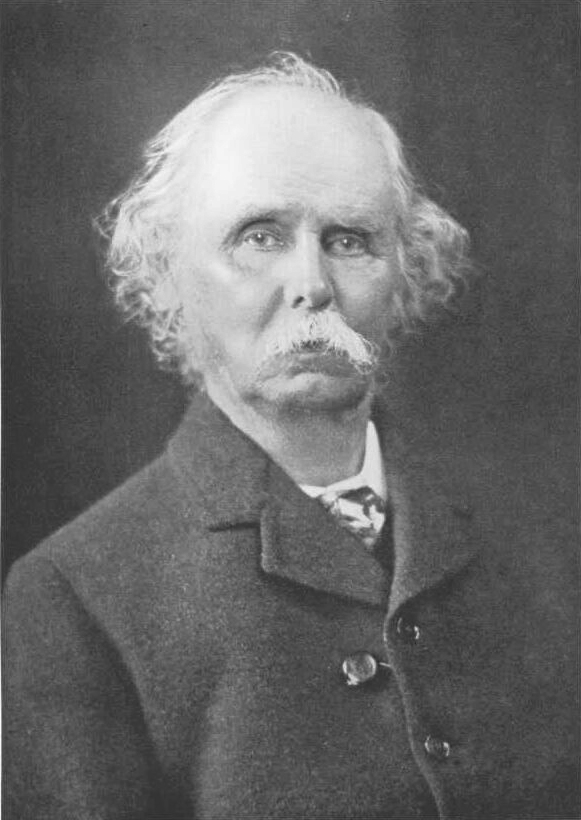
\includegraphics[width=0.5\textwidth]{Alfred_Marshall.jpg}
	\end{center}
\end{frame}

\begin{frame}
	\frametitle{Modelos Lineares para a Procura: Interpreta\c c\~oes}
	\begin{center}
		\begin{tikzpicture}[
			scale = .8,
			every node/.style = {scale=.8},
			declare function = {d(\x)=4-\x;}
		]

			\draw[->] (-0.1,0) -- (5.1,0)node[below right] {$X$};
			\draw[->] (0,-0.1) -- (0,5.1)node[above left] {$p_x$};

			\draw[blue,thick,domain=0:4,variable=\x] plot (\x,{d(\x)});
			\draw(0,4) node[left]{$\frac{a}{b}$};
			\draw(4,0) node[below]{$a$};

			\draw[dashed](2,0) node[below]{$q_1$} -- (2,{d(2)})node[circle,fill,inner sep=1.5pt]{} -- (0,{d(2)}) node[left]{$p_1$};

			\draw(3,1) node[above right]{$D$};
			\draw(3,3) node[above]{$q=a-b\times p$};

		\end{tikzpicture}
	\end{center}

	Para adquirir $q_1$, no m\'aximo os consumidores est\~ao dispostos a pagar $p_1$ por unidade... ou

	Ao pre\c co $p_1$, a escolha \'optima de consumo \'e $q_1$ (individual ou somat\'orio das individuais...)

\end{frame}

\begin{frame}
	\frametitle{Modelos Lineares para a Procura: Interpreta\c c\~oes}
	\begin{center}
		\begin{tikzpicture}[
			scale = .8,
			every node/.style = {scale=.8},
			declare function = {d(\x)=4-\x;}
		]

			\draw[->] (-0.1,0) -- (5.1,0)node[below right] {$X$};
			\draw[->] (0,-0.1) -- (0,5.1)node[above left] {$p_x$};

			\draw[blue,thick,domain=0:4,variable=\x] plot (\x,{d(\x)});
			\draw(0,4) node[left]{$\frac{a}{b}$};
			\draw(4,0) node[below]{$a$};

			\draw[dashed](2,0) node[below]{$q_1$} -- (2,{d(2)})node[circle,fill,inner sep=1.5pt]{} -- (0,{d(2)}) node[left]{$p_1$};

			\draw(3,1) node[above right]{$D$};
			\draw(3,3) node[above]{$q=a-b\times p$};

			\only<2>{
				\draw[red,fill](0,0) -- (2,0) -- (2,{d(2)}) -- (0,{d(2)}) -- (0,0);
			}
			\only<3>{
				\draw[green,fill](0,{d(2)}) -- (0,4) -- (2,{d(2)}) -- (0,{d(2)});
			}

		\end{tikzpicture}
	\end{center}
	{\footnotesize
	\begin{itemize}
		\item $p_1\times q_1$ corresponde \'a {\color{red} despesa} de consumo do bem em an\'alise;
		\item $\left(\frac{a}{b}-p_1\right)\times q_1 \times\frac{1}{2}$ corresponde ao {\color{green} excedente} do consumidor, ou seja corresponde \`a \'area do triangulo acima de $p_1$ e abaixo da Procura.
	\end{itemize}
	}
\end{frame}

\begin{frame}
	\frametitle{Excedente do Consumidor}
	Por unidade do bem transaccionado, \'e a diferen\c ca entre o que o consumidor paga por unidade e o m\'aximo que estaria disposto a pagar (pre\c co de reserva, dado pela procura inversa)...

	\vspace{1cm}

	O excedente total do consumidor num mecado \'e o somat\'orio de todos os excedentes individuais e corresponde graficamente \`a \'area abaixo da curva de procura e acima do pre\c co de mercado.
\end{frame}
\section{Procura Individual - Hicks}
\begin{frame}
	\frametitle{Modelos Lineares para a Procura: Exemplo}
	{\color{blue} Procura \textbf{individual} de p\~ao sem gl\'uten}

	\vspace{0.2cm}
	
	\begin{columns}
		\begin{column}{0.28\textwidth}
			{\color{red}Quadro:}\vspace{0.2cm}
			\begin{tabular}{|c|c|}
				\hline
				Pre\c co & Quantidade \\
				\hline
				0 & 50 \\
				1 & 40 \\
				2 & 30 \\
				3 & 20 \\
				4 & 10 \\
				5 & 0 \\ \hline
			\end{tabular}
			\only<4>{
				Declive da reta?
				\[\frac{d p}{d Q}=\frac{\Delta p}{\Delta Q}=-0.1\]
			}
		\end{column}
		\begin{column}{0.68\textwidth}
		\begin{tabular}{rc}
			{\color{red}Equa\c c\~ao:}& \(Q^D = 50 - 10\times P\)  \\
								ou	  &	\(P = 5 - \frac{1}{10}Q^D\)\\
			{\color{red}Gr\'afico:}	&
		\end{tabular}
		
		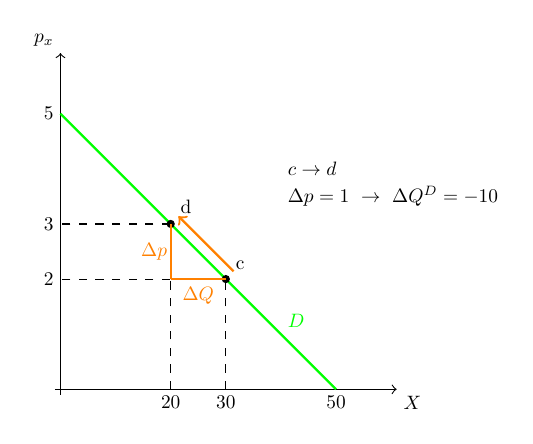
\begin{tikzpicture}[
			scale = 0.7,
			every node/.style = {scale=0.7},
			declare function = {d(\x)=5-\x;}
			]

			\draw[->] (-0.1,0) -- (6.1,0)node[below right] {$X$};
			\draw[->] (0,-0.1) -- (0,6.1)node[above left] {$p_x$};

			\draw[domain=0:5,variable=\x,green,thick] plot (\x,{d(\x)});
			\draw(4,{d(4)}) node[green,above right]{$D$};
			\draw(0,{d(0)}) node[left]{5};
			\draw(5,0) node[below]{50};

			\onslide<2-3>{
				\draw[dashed](3,0) node[below]{30} -- (3,{d(3)})node[circle,fill,inner sep=1.5pt,label=above right:c]{} -- (0,{d(3)}) node[left]{2};
				\draw[dashed](2,0) node[below]{20} -- (2,{d(2)})node[circle,fill,inner sep=1.5pt,label=above right:d]{} -- (0,{d(2)}) node[left]{3};
				\draw(4,4) node[right]{\(c\rightarrow d\)};
			}

			\onslide<3-4>{
				\draw[->,thick,orange] (3+0.14,{d(3)+0.14}) -- (2+0.14,{d(2)+0.14});
				\draw(4,3.5) node[right]{\(\Delta p = 1 \ \rightarrow\ \Delta Q^D=-10\)};
				\draw[thick,orange](2,{d(3)})--(3,{d(3)})node[midway,yshift=-0.3cm]{$\Delta Q$};
				\draw[thick,orange](2,{d(2)})--(2,{d(3)})node[midway,xshift=-0.3cm]{$\Delta p$};
			}

		\end{tikzpicture}
		\end{column}
	\end{columns}
\end{frame}

\begin{frame}
	\frametitle{Modelos Lineares para a procura: Exemplo}
	{\color{blue} Procura \textbf{de mercado} de p\~ao sem gl\'uten: N=2}

	\vspace{0.2cm}
	
	\begin{columns}

		\begin{column}{0.25\textwidth}
		{\footnotesize
		{\color{green}Consumidor 1}\\
		\(Q_1^D=50-10\times p\)
		\(P=5-0.1\times Q\)
		}
		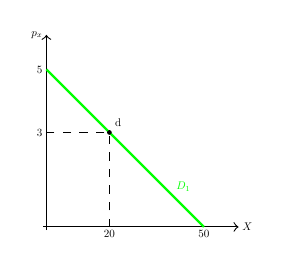
\begin{tikzpicture}[
			scale = 0.4,
			every node/.style = {scale=0.4},
			declare function = {d(\x)=5-\x;}
			]

			\draw[->] (-0.1,0) -- (6.1,0)node[right] {$X$};
			\draw[->] (0,-0.1) -- (0,6.1)node[left] {$p_x$};

			\draw[domain=0:5,variable=\x,green,thick] plot (\x,{d(\x)});
			\draw(4,{d(4)}) node[green,above right]{$D_1$};
			\draw(0,{d(0)}) node[left]{5};
			\draw(5,0) node[below]{50};

			\draw[dashed](2,0) node[below]{20} -- (2,{d(2)})node[circle,fill,inner sep=1.5pt,label=above right:d]{} -- (0,{d(2)}) node[left]{3};

		\end{tikzpicture}
		\end{column}
		
		\begin{column}{0.25\textwidth}
		{\footnotesize
		{\color{red}Consumidor 2}\\
		\(Q_2^D=50-10\times p\)
		\(P=5-0.1\times Q\)
		}
		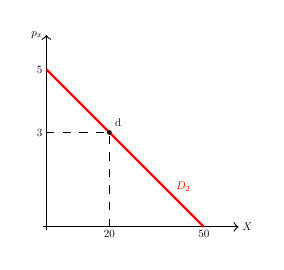
\begin{tikzpicture}[
			scale = 0.4,
			every node/.style = {scale=0.4},
			declare function = {d(\x)=5-\x;}
			]

			\draw[->] (-0.1,0) -- (6.1,0)node[right] {$X$};
			\draw[->] (0,-0.1) -- (0,6.1)node[left] {$p_x$};

			\draw[domain=0:5,variable=\x,red,thick] plot (\x,{d(\x)});
			\draw(4,{d(4)}) node[red,above right]{$D_2$};
			\draw(0,{d(0)}) node[left]{5};
			\draw(5,0) node[below]{50};

			\draw[dashed](2,0) node[below]{20} -- (2,{d(2)})node[circle,fill,inner sep=1.5pt,label=above right:d]{} -- (0,{d(2)}) node[left]{3};

		\end{tikzpicture}
		\end{column}
		\begin{column}{0.5\textwidth}
		{\footnotesize
		{\color{blue}Mercado}\\
		\(Q_M^D=100-20\times p\)\\
		\(P=5-0.05\times Q\)
		}
		\begin{tikzpicture}[
			scale = 0.4,
			every node/.style = {scale=0.4},
			declare function = {d(\x)=5-0.5*\x;}
			]

			\draw[->] (-0.1,0) -- (11.1,0)node[right] {$X$};
			\draw[->] (0,-0.1) -- (0,6.1)node[left] {$p_x$};

			\draw[domain=0:10,variable=\x,blue,thick] plot (\x,{d(\x)});
			\draw(8,{d(8)}) node[blue,above right]{$D_{mercado}$};
			\draw(0,{d(0)}) node[left]{5};
			\draw(10,0) node[below]{100};

			\draw[dashed](4,0) node[below]{40} -- (4,{d(4)})node[circle,fill,inner sep=1.5pt,label=above right:d]{} -- (0,{d(4)}) node[left]{3};

		\end{tikzpicture}
		\end{column}
	\end{columns}
	\vspace{0.4cm}
	A agrega\c c\~ao \'e sempre horizontal: O que se adiciona s\~ao quantidades, n\~ao pre\c cos. Se juntamos dois consumidores iguais, n\~ao \'e a mesma quantidade ao dobro do pre\c co, mas sim o dobro da quantidade ao mesmo pre\c co!!!
\end{frame}


\begin{frame}
	\frametitle{Curva de Procura Individual e altera\c c\~oes de rendimento}
	\begin{center}
			\def\rho{0.5}
			\def\ww{10}
			\def\whw{22}
			\def\pyy{3}
			\def\pxx{3}
			\begin{tikzpicture}[
				scale = 0.8,
				every node/.style={scale = 0.8},
				declare function={
					x(\w,\px,\py) = (\w*(\px^(1/(\rho-1))))/(\px^(\rho/(\rho-1))+\py^(\rho/(\rho-1)));
					y(\w,\px,\py) = (\w*(\py^(1/(\rho-1))))/(\px^(\rho/(\rho-1))+\py^(\rho/(\rho-1)));
					u(\x,\y) = (\x^\rho+\y^\rho)^(1/\rho);
					ic(\w,\x,\px,\py) = (u(x(\w,\px,\py),y(\w,\px,\py))^\rho-\x^\rho)^(1/\rho);
					bc(\w,\x,\px,\py) = \w/\py - (\px/\py)*\x;
				}
				]

				\draw[->] (-0.1,0) -- (8.1,0)node[below right] {$X$};
				\draw[->] (0,-0.1) -- (0,8.1)node[above left] {$Y$};

				\draw[samples=100,blue,domain=0:(10/\pxx),variable=\x] plot (\x,{bc(10,\x,\pxx,\pyy)});
				\draw({10/\pxx},0) node[circle,fill,inner sep=1.5pt,label=below :\(\frac{W}{p_x}\)]{};
				\draw(0,{10/\pyy}) node[circle,fill,inner sep=1.5pt,label=left :\(\frac{W}{p_y}\)]{};
				\draw[samples=100,red,domain=.70:5,variable=\x] plot (\x,{ic(10,\x,\pxx,\pyy)});
				\draw({x(10,\pxx,\pyy)},{y(10,\pxx,\pyy)}) node[red,circle,fill,inner sep=1.5pt]{};

				\onslide<2->{
					\draw[->,blue,thick] (0,2) -- (4,6) node[above right]{\parbox[l]{3cm}{Aumento de $W$}};
					\draw[samples=100,blue,domain=0:(15/\pxx),variable=\x] plot (\x,{bc(15,\x,\pxx,\pyy)});
					\draw({15/\pxx},0) node[circle,fill,inner sep=1.5pt,label=below :\(\frac{W'}{p_x}\)]{};
					\draw(0,{15/\pyy}) node[circle,fill,inner sep=1.5pt,label=left :\(\frac{W'}{p_y}\)]{};
					\draw[samples=100,red,domain=.70:5,variable=\x] plot (\x,{ic(15,\x,\pxx,\pyy)});
					\draw({x(15,\pxx,\pyy)},{y(15,\pxx,\pyy)}) node[red,circle,fill,inner sep=1.5pt]{};				
				}

				\onslide<3->{
					\draw[samples=100,blue,domain=0:(20/\pxx),variable=\x] plot (\x,{bc(20,\x,\pxx,\pyy)});
					\draw({20/\pxx},0) node[circle,fill,inner sep=1.5pt,label=below :\(\frac{W''}{p_x}\)]{};
					\draw(0,{20/\pyy}) node[circle,fill,inner sep=1.5pt,label=left :\(\frac{W''}{p_y}\)]{};
					\draw[samples=100,red,domain=.70:5,variable=\x] plot (\x,{ic(20,\x,\pxx,\pyy)});
					\draw({x(20,\pxx,\pyy)},{y(20,\pxx,\pyy)}) node[red,circle,fill,inner sep=1.5pt]{};				
				}

				\onslide<4->{
					\draw[thick,green] plot[smooth,tension=0.4] coordinates{(0,0) (1.4,1.2) ({x(10,\pxx,\pyy)},{y(10,\pxx,\pyy)}) ({x(15,\pxx,\pyy)},{y(15,\pxx,\pyy)}) ({x(20,\pxx,\pyy)},{y(20,\pxx,\pyy)}) (5,5.5)} node[black,below right]{\parbox[l]{3cm}{Via de Expans\~ao do Rendimento}};
				}

			\end{tikzpicture}
		\end{center}
\end{frame}

\begin{frame}
	\frametitle{Via de Expans\~ao de Rendimento e Curvas de Engel (bens normais)}
		\begin{center}
			\def\rho{0.5}
			\def\pyy{3}
			\def\pxx{3}
			\begin{tikzpicture}[
				scale = 0.4,
				every node/.style={scale = 0.4},
				declare function={
					x(\w,\px,\py) = (\w*(\px^(1/(\rho-1))))/(\px^(\rho/(\rho-1))+\py^(\rho/(\rho-1)));
					y(\w,\px,\py) = (\w*(\py^(1/(\rho-1))))/(\px^(\rho/(\rho-1))+\py^(\rho/(\rho-1)));
					u(\x,\y) = (\x^\rho+\y^\rho)^(1/\rho);
					ic(\w,\x,\px,\py) = (u(x(\w,\px,\py),y(\w,\px,\py))^\rho-\x^\rho)^(1/\rho);
					bc(\w,\x,\px,\py) = \w/\py - (\px/\py)*\x;
				}
				]

				\draw[->] (-0.1,0) -- (8.1,0)node[below right] {$X$};
				\draw[->] (0,-0.1) -- (0,8.1)node[above left] {$Y$};

				\draw[samples=100,blue,domain=0:(10/\pxx),variable=\x] plot (\x,{bc(10,\x,\pxx,\pyy)});
				\draw({10/\pxx},0) node[circle,fill,inner sep=1.5pt,label=below :\(\frac{W}{p_x}\)]{};
				\draw(0,{10/\pyy}) node[circle,fill,inner sep=1.5pt,label=left :\(\frac{W}{p_y}\)]{};
				\draw[samples=100,red,domain=.70:5,variable=\x] plot (\x,{ic(10,\x,\pxx,\pyy)});
				\draw({x(10,\pxx,\pyy)},{y(10,\pxx,\pyy)}) node[red,circle,fill,inner sep=1.5pt]{};

				\draw[->,blue,thick] (0,2) -- (4,6) node[above right]{\parbox[l]{3cm}{Aumento de $W$}};
				\draw[samples=100,blue,domain=0:(15/\pxx),variable=\x] plot (\x,{bc(15,\x,\pxx,\pyy)});
				\draw({15/\pxx},0) node[circle,fill,inner sep=1.5pt,label=below :\(\frac{W'}{p_x}\)]{};
				\draw(0,{15/\pyy}) node[circle,fill,inner sep=1.5pt,label=left :\(\frac{W'}{p_y}\)]{};
				\draw[samples=100,red,domain=.70:5,variable=\x] plot (\x,{ic(15,\x,\pxx,\pyy)});
				\draw({x(15,\pxx,\pyy)},{y(15,\pxx,\pyy)}) node[red,circle,fill,inner sep=1.5pt]{};				

				\draw[samples=100,blue,domain=0:(20/\pxx),variable=\x] plot (\x,{bc(20,\x,\pxx,\pyy)});
				\draw({20/\pxx},0) node[circle,fill,inner sep=1.5pt,label=below :\(\frac{W''}{p_x}\)]{};
				\draw(0,{20/\pyy}) node[circle,fill,inner sep=1.5pt,label=left :\(\frac{W''}{p_y}\)]{};
				\draw[samples=100,red,domain=.70:5,variable=\x] plot (\x,{ic(20,\x,\pxx,\pyy)});
				\draw({x(20,\pxx,\pyy)},{y(20,\pxx,\pyy)}) node[red,circle,fill,inner sep=1.5pt]{};				

				\draw[green] plot[smooth,tension=0.4] coordinates{(0,0) (1.4,1.2) ({x(10,\pxx,\pyy)},{y(10,\pxx,\pyy)}) ({x(15,\pxx,\pyy)},{y(15,\pxx,\pyy)}) ({x(20,\pxx,\pyy)},{y(20,\pxx,\pyy)}) (5,5.5)} node[black,below right]{\parbox[l]{3cm}{Via de Expans\~ao do Rendimento}};

				\draw[->] (-0.1,-8) -- (8.1,-8)node[below right] {$X$};
				\draw[->] (0,-8.1) -- (0,-1.9)node[above left] {$W$};

				\onslide<3->{
					\draw[dotted] (0,{1-8}) node[left]{10} -- ({x(10,\pxx,\pyy)},{1-8});
					\draw[dotted] (0,{1.5-8}) node[left]{15} -- ({x(15,\pxx,\pyy)},{1.5-8});
					\draw[dotted] (0,{2-8}) node[left]{20} -- ({x(20,\pxx,\pyy)},{2-8});
				}

				\onslide<2->{
					\draw[dotted] ({x(10,\pxx,\pyy)},-8) -- ({x(10,\pxx,\pyy)},{y(10,\pxx,\pyy)});
					\draw[dotted] ({x(15,\pxx,\pyy)},-8) -- ({x(15,\pxx,\pyy)},{y(15,\pxx,\pyy)});
					\draw[dotted] ({x(20,\pxx,\pyy)},-8) -- ({x(20,\pxx,\pyy)},{y(20,\pxx,\pyy)});	
				}

				\onslide<4->{
					\draw[thick,green] plot[smooth,tension=0.4] coordinates{
						(0,-8)
						(1.4,{1.0-8})
						({x(10,\pxx,\pyy)},{1-8})
						({x(15,\pxx,\pyy)},{1.5-8})
						({x(20,\pxx,\pyy)},{2.0-8})
						(5,{3.5-8})
						} node[black,below right]{\parbox[l]{3cm}{Curva de Engel do Bem \(x\)}};
				}

			\end{tikzpicture}
		\end{center}
\end{frame}

\begin{frame}
	\frametitle{Caso o bem $X$ seja um bem inferior}
		\begin{center}
			\def\rho{0.5}
			\def\pyy{3}
			\def\pxx{3}
			\begin{tikzpicture}[
				scale = 0.4,
				every node/.style={scale = 0.4},
				declare function={
					x(\w,\px,\py) = (\w*(\px^(1/(\rho-1))))/(\px^(\rho/(\rho-1))+\py^(\rho/(\rho-1)));
					y(\w,\px,\py) = (\w*(\py^(1/(\rho-1))))/(\px^(\rho/(\rho-1))+\py^(\rho/(\rho-1)));
					u(\x,\y) = (\x^\rho+\y^\rho)^(1/\rho);
					ic(\w,\x,\px,\py) = (u(x(\w,\px,\py),y(\w,\px,\py))^\rho-\x^\rho)^(1/\rho);
					ic2(\w,\x,\px,\py) = (u(x(\w,\px,\py),y(\w,\px,\py))^\rho-\x^\rho)^(1/\rho)+3;
					bc(\w,\x,\px,\py) = \w/\py - (\px/\py)*\x;
				}
				]

				\draw[->] (-0.1,0) -- (8.1,0)node[below right] {$X$};
				\draw[->] (0,-0.1) -- (0,8.1)node[above left] {$Y$};

				\draw[samples=100,blue,domain=0:(10/\pxx),variable=\x] plot (\x,{bc(10,\x,\pxx,\pyy)});
				\draw({10/\pxx},0) node[circle,fill,inner sep=1.5pt,label=below :\(\frac{W}{p_x}\)]{};
				\draw(0,{10/\pyy}) node[circle,fill,inner sep=1.5pt,label=left :\(\frac{W}{p_y}\)]{};
				\draw[samples=100,red,domain=.70:5,variable=\x] plot (\x,{ic(10,\x,\pxx,\pyy)});
				\draw({x(10,\pxx,\pyy)},{y(10,\pxx,\pyy)}) node[red,circle,fill,inner sep=1.5pt]{};

				\draw[->,blue,thick] (0,2) -- (4,6) node[above right]{\parbox[l]{3cm}{Aumento de $W$}};
				\draw[samples=100,blue,domain=0:(15/\pxx),variable=\x] plot (\x,{bc(15,\x,\pxx,\pyy)});
				\draw({15/\pxx},0) node[circle,fill,inner sep=1.5pt,label=below :\(\frac{W'}{p_x}\)]{};
				\draw(0,{15/\pyy}) node[circle,fill,inner sep=1.5pt,label=left :\(\frac{W'}{p_y}\)]{};
				\draw[samples=100,red,domain=.70:5,variable=\x] plot (\x,{ic(15,\x,\pxx,\pyy)});
				\draw({x(15,\pxx,\pyy)},{y(15,\pxx,\pyy)}) node[red,circle,fill,inner sep=1.5pt]{};				

				\draw[samples=100,blue,domain=0:(20/\pxx),variable=\x] plot (\x,{bc(20,\x,\pxx,\pyy)});
				\draw({20/\pxx},0) node[circle,fill,inner sep=1.5pt,label=below :\(\frac{W''}{p_x}\)]{};
				\draw(0,{20/\pyy}) node[circle,fill,inner sep=1.5pt,label=left :\(\frac{W''}{p_y}\)]{};
				\draw[samples=100,red,domain=.80:5,variable=\x] plot (\x,{ic2(11,\x,\pxx,\pyy)});
				\draw({x(11,\pxx,\pyy)},{ic2(11,x(11,\pxx,\pyy),\pxx,\pyy)}) node[red,circle,fill,inner sep=1.5pt]{};				

				\draw[thick,green] plot[smooth,tension=0.4] coordinates{
					(0,0)
					(1.4,1.2)
					({x(10,\pxx,\pyy)},{y(10,\pxx,\pyy)})
					({x(15,\pxx,\pyy)},{y(15,\pxx,\pyy)})
					({x(11,\pxx,\pyy)},{ic2(11,x(11,\pxx,\pyy),\pxx,\pyy)})
					(1.55,5.5)
				} node[black,above]{\parbox[l]{3cm}{Via de Expans\~ao do Rendimento}};

				\draw[->] (-0.1,-8) -- (8.1,-8)node[below right] {$X$};
				\draw[->] (0,-8.1) -- (0,-1.9)node[above left] {$W$};

				\draw[dotted] (0,{1-8}) node[left]{10} -- ({x(10,\pxx,\pyy)},{1-8});
				\draw[dotted] (0,{1.5-8}) node[left]{15} -- ({x(15,\pxx,\pyy)},{1.5-8});
				\draw[dotted] (0,{2-8}) node[left]{20} -- ({x(11,\pxx,\pyy)},{2-8});

				\draw[dotted] ({x(10,\pxx,\pyy)},-8) -- ({x(10,\pxx,\pyy)},{y(10,\pxx,\pyy)});
				\draw[dotted] ({x(15,\pxx,\pyy)},-8) -- ({x(15,\pxx,\pyy)},{y(15,\pxx,\pyy)});
				\draw[dotted] ({x(11,\pxx,\pyy)},-8) -- ({x(11,\pxx,\pyy)},{ic2(11,x(11,\pxx,\pyy),\pxx,\pyy)});	

				\draw[thick,green] plot[smooth,tension=0.4] coordinates{
						(0,-8)
						(1.4,{1.0-8})
						({x(10,\pxx,\pyy)},{1-8})
						({x(15,\pxx,\pyy)},{1.5-8})
						({x(11,\pxx,\pyy)},{2.0-8})
						(1,{2.5-8})
					} node[black,below right]{\parbox[l]{3cm}{Curva de Engel do Bem \(x\)}};

			\end{tikzpicture}
		\end{center}
\end{frame}


\begin{frame}
	\frametitle{Lei da Procura}
	Voltemos \`a rela\c c\~ao negativa entre quantidade procurada de um bem e pre\c co desse mesmo bem!

	\vspace{0.5cm}

	A rela\c c\~ao fiocu demonstrada graficamente, mas quais as raz\~oes efectivas para esta conclus\~ao?

	\vspace{0.4cm}

	Vejamos...
\end{frame}

\begin{frame}
	\frametitle{Lei da Procura}
	\begin{center}
	\LARGE A altera\c c\~ao no pre\c co do bem leva a uma altera\c c\~ao do seu consumo devido a dois efeitos:
	\end{center}
\end{frame}

\begin{frame}
	\frametitle{Efeito Substitui\c c\~ao e Efeito Rendimento ap\'os $\Delta p$}

	\textbf{\underline{Efeito substitui\c c\~ao:}} se o pre\c co de um bem aumenta (\emph{c\ae teris paribus}), a quantidade procurada diminui porque os consumidores olham para alternativas que satisfa\c cam a mesma necessidade, passando alguns deles a adquirir esses bens substitutos
\end{frame}

\begin{frame}
	\frametitle{Efeito Substitui\c c\~ao e Efeito Rendimento ap\'os $\Delta p$}
	\textbf{\underline{Efeito rendimento:}} se o pre\c co de um bem aumenta (\emph{c\ae teris paribus}), a quantidade procurada diminui porque os consumidores se sentem mais pobres com o \textbf{\underline{mesmo rendimento}} e reduzem o seu consumo (quebra de poder de compra)

	\vspace{1cm}

	Nota: Efeito rendimento $\neq$ Altera\c c\~oes no rendimento
\end{frame}

\begin{frame}
	\frametitle{Efeitos substitui\c c\~ao (Hicks) e Rendimento (x bem normal)}
	\begin{center}
			\def\rho{0.5}
			\def\pxx{3}
			\def\pyy{3}
			\def\qxx{5}
			\def\qyy{4}
			\begin{tikzpicture}[
				scale = 0.7,
				every node/.style={scale = 0.7},
				declare function={
					x(\w,\px,\py) = (\w*(\px^(1/(\rho-1))))/(\px^(\rho/(\rho-1))+\py^(\rho/(\rho-1)));
					y(\w,\px,\py) = (\w*(\py^(1/(\rho-1))))/(\px^(\rho/(\rho-1))+\py^(\rho/(\rho-1)));
					u(\x,\y) = (\x^\rho+\y^\rho)^(1/\rho);
					ic(\w,\x,\px,\py) = (u(x(\w,\px,\py),y(\w,\px,\py))^\rho-\x^\rho)^(1/\rho);
					bc(\w,\x,\px,\py) = \w/\py - (\px/\py)*\x;
				}
				]

				\draw[->] (-0.1,0) -- (8.1,0)node[below right] {$X$};
				\draw[->] (0,-0.1) -- (0,8.1)node[above left] {$Y$};

				\draw[samples=100,blue,domain=0:(20/\pxx),variable=\x] plot (\x,{bc(20,\x,\pxx,\pyy)});
				\draw({20/\pxx},0) node[circle,fill,inner sep=1.5pt,label=below :\(\frac{W}{p_x}\)]{};
				\draw(0,{20/\pyy}) node[circle,fill,inner sep=1.5pt,label=left :\(\frac{W}{p_y}\)]{};
				\draw[samples=100,red,domain=.9:6,variable=\x] plot (\x,{ic(20,\x,\pxx,\pyy)});
				\draw({x(20,\pxx,\pyy)},{y(20,\pxx,\pyy)}) node[red,circle,fill,inner sep=1.5pt,label=above right:{\(A^*(P,W)\)}]{};
				
				\onslide<2->{
					\draw[samples=100,blue,domain=0:(20/\qxx),variable=\x] plot (\x,{bc(20,\x,\qxx,\pyy)});
					\draw({20/\qxx},0) node[circle,fill,inner sep=1.5pt,label=below :\(\frac{W}{p_x'}\)]{};
					\draw(0,{20/\pyy}) node[circle,fill,inner sep=1.5pt,label=left :\(\frac{W}{p_y}\)]{};
					\draw[samples=100,red,domain=.65:5,variable=\x] plot (\x,{ic(20,\x,\qxx,\pyy)});
					\draw({x(20,\qxx,\pyy)},{y(20,\qxx,\pyy)}) node[red,circle,fill,inner sep=1.5pt,label=below left:{\(A^*(P',W)\)}]{};
				}

				\onslide<3->{
					\draw[samples=100,green,thick,domain=0:(20/\qxx),variable=\x] plot (\x,{bc(25,\x,\qxx,\pyy)});
					\draw(2,5) node[red,circle,fill,inner sep=1.5pt,label=above right:{\(A^s\)}]{};
				}

				\onslide<4->{
					\draw[->,thick] ({x(20,\pxx,\pyy)},{y(20,\pxx,\pyy)}) -- (2,{y(20,\pxx,\pyy)}) node[below right]{Efeito Substitui\c c\~ao};
					\draw[dotted] ({x(20,\pxx,\pyy)},0) -- ({x(20,\pxx,\pyy)},{y(20,\pxx,\pyy)});
					\draw[dotted] (2,0) -- (2,5);
				}

				\onslide<4->{
					\draw[->,thick,brown] (2,{y(20,\pxx,\pyy)}) -- ({x(20,\qxx,\pyy)},{y(20,\pxx,\pyy)}) node[below left]{Efeito Rendimento};
					\draw[dotted] ({x(20,\qxx,\pyy)},0) -- ({x(20,\qxx,\pyy)},{y(20,\qxx,\pyy)});
				}


			\end{tikzpicture}
	\end{center}
\end{frame}

\begin{frame}
	\frametitle{Exemplo da abordagem Hicksiana}
	\begin{itemize}
		\item Prefer\^encias descritas por $u(x,y)=0.8 \ln x + 0.2 \ln y$
		\item Or\c camento dispon\'ivel de 100u.m.
		\item $p_x=8$; $p_y=2$, inicialmente
		\item Alterar para $p_x=10$ u.m. \emph{c\ae teris paribus}
	\end{itemize}
\end{frame}

\begin{frame}
	\frametitle{Abordagem Hicksiana}
	\[|TMS|=\frac{4y}{x}\]
	Aos novos pre\c cos, a 2\textsuperscript{a} lei de Gossen obriga a:\\
	\[\frac{4y}{x}=5\]
	A  utilidade do cabaz inicial \'e 2.3, o que quer dizer que o cabaz separador de Hicks \'e tal que: \[2.3 = 0.8\ln{x}+0.2\ln{y}\] e em simult\^aneo tem de se cumprir que \(\frac{4y}{x}=5\), o que configura um sistema de duas equa\c c\~oes com duas inc\'ognitas cuja solu\c c\~ao devolve o ponto $A^s$.
\end{frame}

\begin{frame}
	\frametitle{Exemplo da abordagem Hicksiana}
	{\footnotesize
	\renewcommand{\arraystretch}{2}
	\begin{tabular}{cccc}
	& Inicial & Separador de Hicks & Final \\ \hline
	Escolha \'optima & $x=y=10$ & $x=9.56$; $y=11.95$ & $x=8$; $y=10$\\
	R\'acio de pre\c cos & 4 & 5 & 5 \\
	Despesa de consumo & 100 & 119.54 & 100 \\
	Utilidade da escolha & 2.3 & 2.3 & 2.12
	\end{tabular}
	}

	\vspace{0.5cm}

	Para o consumidor ter a mesma utilidade que tinha antes do aumento de pre\c co, seria necess\'ario receber uma compensa\c c\~ao de 19.54 u.m. (Varia\c c\~ao Compensat\'oria)
\end{frame}

\begin{frame}
	\frametitle{Exemplo}
	\begin{center}
			\def\rho{0.5}
			\def\pxx{1}
			\def\pyy{1}
			\def\qxx{4}
			\def\qyy{1}
			\begin{tikzpicture}[
				scale = 1,
				every node/.style={scale = 0.7},
				declare function={
					%x(\w,\px,\py) = (\w*(\px^(1/(\rho-1))))/(\px^(\rho/(\rho-1))+\py^(\rho/(\rho-1))); %CES
					%y(\w,\px,\py) = (\w*(\py^(1/(\rho-1))))/(\px^(\rho/(\rho-1))+\py^(\rho/(\rho-1))); %CES
					%u(\x,\y) = (\x^\rho+\y^\rho)^(1/\rho); %CES
					%ic(\w,\x,\px,\py) = (u(x(\w,\px,\py),y(\w,\px,\py))^\rho-\x^\rho)^(1/\rho); %CES
					x(\w,\px,\py) = (\w*\rho)/\px; %Cobb-Douglas
					y(\w,\px,\py) = (\w*(1-\rho))/\py; %Cobb-Douglas
					u(\x,\y) = \x^(\rho)*\y^(1-\rho); %Cobb-Douglas
					ic(\w,\x,\px,\py) = (v(\w,\px,\py)/(\x^\rho))^(1/(1-\rho)); %Cobb-Douglas
					v(\w,\px,\py) = u(x(\w,\px,\py),y(\w,\px,\py));
					bc(\w,\x,\px,\py) = \w/\py - (\px/\py)*\x;
				}
				]

				\draw[->] (-0.1,0) -- (5.5,0)node[below right] {$X$};
				\draw[->] (0,-0.1) -- (0,5.5)node[above left] {$Y$};

				\onslide<2->{
					\draw[samples=100,blue,domain=0:(5/\pxx),variable=\x] plot (\x,{bc(5,\x,\pxx,\pyy)});
					\draw({5/\pxx},0) node[circle,fill,inner sep=1.5pt,label=below :\(\frac{W}{p_x}\)]{};
					\draw(0,{5/\pyy}) node[circle,fill,inner sep=1.5pt,label=left :\(\frac{W}{p_y}\)]{};
					\draw[samples=50,red,domain=1.1:5,variable=\x] plot (\x,{ic(5,\x,\pxx,\pyy)}) node[right]{\(u=2.3\)};
					\draw({x(5,\pxx,\pyy)},{y(5,\pxx,\pyy)}) node[blue,circle,fill,inner sep=1.5pt]{};
					\draw(0,{y(5,\pxx,\pyy)}) node[circle,fill,inner sep=1.5pt,label=left:{\(10\)}]{};
					\draw({x(5,\pxx,\pyy)},0) node[circle,fill,inner sep=1.5pt,label=below:{\(10\)}]{};
				}

				\onslide<3->{
					\draw[samples=100,blue,domain=0:(5/\qxx),variable=\x] plot (\x,{bc(5,\x,\qxx,\pyy)});
					\draw[samples=50,red,domain=0.45:5,variable=\x] plot (\x,{ic(5,\x,\qxx,\pyy)}) node[right]{\(u=2.12\)};
					\draw({x(5,\qxx,\pyy)},{y(5,\qxx,\pyy)}) node[blue,circle,fill,inner sep=1.5pt]{};
					\draw({x(5,\qxx,\pyy)},0) node[circle,fill,inner sep=1.5pt,label=below:{\(8\)}]{};
				}

				\only<3>{
					\draw[->,thick] ({x(5,\pxx,\pyy)},{y(5,\pxx,\pyy)}) -- ({x(5,\qxx,\pyy)},{y(5,\qxx,\pyy)}) node[midway,yshift=-7]{Ef.Total};
				}

				\onslide<4->{
					\draw[samples=100,green,domain=0.9:(10/\qxx),variable=\x] plot (\x,{bc(10,\x,\qxx,\pyy)});
					\draw({x(10,\qxx,\pyy)},{y(10,\qxx,\pyy)}) node[black,circle,fill,inner sep=1.5pt,label=right:{Despesa \(119.54\) u.m.}]{};
					\draw({x(10,\qxx,\pyy)},0) node[circle,fill,inner sep=1.5pt,label=below:\(9.56\)]{};
				}

				\onslide<5->{
					\draw[dotted] ({x(5,\pxx,\pyy)},0) -- ({x(5,\pxx,\pyy)},{y(5,\pxx,\pyy)});
					\draw[dotted] ({x(5,\qxx,\pyy)},0) -- ({x(5,\qxx,\pyy)},{y(5,\qxx,\pyy)});
					\draw[dotted] ({x(10,\qxx,\pyy)},0) -- ({x(10,\qxx,\pyy)},{y(10,\qxx,\pyy)});	
				}

				\onslide<6->{
					\draw[->,thick] ({x(5,\pxx,\pyy)},-0.42) -- ({x(10,\qxx,\pyy)},-0.42) node[midway,yshift=-7,xshift=5]{Ef.Sub.};
				}

				\onslide<7->{
					\draw[->,thick] ({x(10,\qxx,\pyy)},-0.4) -- ({x(5,\qxx,\pyy)},-0.4) node[midway,yshift=-7,xshift=-5]{Ef.Rend.};	
				}

			\end{tikzpicture}\\
			Nos pontos azuis, a despesa \'e de \(100\) u.m.
	\end{center}
\end{frame}

\begin{frame}
	\frametitle{E para bens inferiores?}
	\begin{itemize}
	\item O efeito rendimento contraria uma parte do efeito substitui\c c\~ao, o que significa que o ponto $A^s(P',W')$ no gr\'afico, est\'a \`a esquerda de $A^*(P',W)$
	\item Para uma certa categoria de bens inferiores, pode at\'e acontecer que o efeito rendimento seja predominante face ao efeito substitui\c c\~ao, ap\'os uma altera\c c\~ao de pre\c co --- Bens de Giffen
	\end{itemize}
\end{frame}

\begin{frame}
	\frametitle{Efeitos substitui\c c\~ao (Hicks) e Rendimento (x bem inferior)}
	\begin{center}	
		\def\a{1}
		\def\from{0.1}
		\def\fixh{-0.1}
		% Utility function for x inferior good, Liebhafsky (AER 1969)
		\begin{tikzpicture}[
			scale = 1.8,
			every node/.style = {scale = 0.7},
			declare function = {
				u(\x,\y) = \a*ln(\x) + (\y^2)/2;
				x(\px,\py,\w) = (1/(2*\px))*(\w-(\w^2-4*\a*(\py^2))^(1/2));
				y(\px,\py,\w) = (1/(2*\py))*(\w+(\w^2-4*\a*(\py^2))^(1/2));
				v(\px,\py,\w) = u(x(\px,\py,\w),y(\px,\py,\w));
				ic(\x,\px,\py,\w) = (2*(v(\px,\py,\w)-\a*ln(\x)))^(1/2);
				bc(\x,\px,\py,\w) = \w/\py - (\px/\py)*\x;
				}
			]

			\draw[->] (0,0) -- (5.2,0) node[below] {$x$};
			\draw[->] (0,0) -- (0,3.2) node[left] {$y$};

			\onslide<2->{
				\draw[domain=0:(5/1),samples=50,variable=\x] plot (\x,{bc(\x,1,2,5)});
				\draw[domain=\from:3,samples=50,variable=\x] plot (\x,{ic(\x,1,2,5)});
				\draw({x(1,2,5)},{y(1,2,5)}) node[circle,fill,inner sep=1.5pt,label=above right:{$A^*(P,W)$}]{};
			}

			\onslide<3->{
				\draw[blue,domain=0:(5/2),samples=50,variable=\x] plot (\x,{bc(\x,2,2,5)});
				\draw[blue,domain=\from:3,samples=50,variable=\x] plot (\x,{ic(\x,2,2,5)});	
				\draw({x(2,2,5)},{y(2,2,5)}) node[circle,fill,inner sep=1.5pt,label=below left:{$A^*(P',W)$}]{};
			}
			
			\onslide<4->{
				\draw[red,domain=0:(5/2),samples=50,variable=\x] plot (\x,{bc(\x,2,2,5)+0.3});
				\draw({x(2,2,5)+\fixh},{ic(x(2,2,5)+\fixh,1,2,5)}) node[red,circle,fill,inner sep=1.5pt,label=above right:{$A^s$}]{};
			}			
			
			\onslide<5->{
				\draw[dotted] ({x(1,2,5)},{y(1,2,5)}) -- ({x(1,2,5)},0);
				\draw[dotted] ({x(2,2,5)},{y(2,2,5)}) -- ({x(2,2,5)},0);
				\draw[dotted] ({x(2,2,5)+\fixh},{ic(x(2,2,5)+\fixh,1,2,5)}) -- ({x(2,2,5)+\fixh},0);
			}

			\onslide<6->{
				\draw[->,red,thick] ({x(1,2,5)},0.25) -- ({x(2,2,5)+\fixh},0.25);			
			}

			\onslide<7->{
				\draw[->,orange,thick] ({x(2,2,5)+\fixh},0.15) -- ({x(2,2,5)},0.15);
			}

		\end{tikzpicture}
	\end{center}
	\onslide<6->{\color{red}Ef. Substitui\c c\~ao (\(\leftarrow\)),} \onslide<7->{\color{orange}Ef. Rendimento (\(\rightarrow\)).}
\end{frame}

\begin{frame}
	\frametitle{Bem de Giffen - excep\c c\~ao \`a Lei da Procura}
	\begin{center}
		\def\duxa{0}
		\def\duya{0}
		\def\duxb{0.5}
		\def\duyb{0.6}
		\def\duxc{-0.95}
		\def\duyc{2}
		\begin{tikzpicture}[
				scale = 0.4,
				every node/.style={scale = 0.5}
			]

				\draw[->] (-0.1,0) -- (9.1,0)node[below right] {$X$};
				\draw[->] (0,-0.1) -- (0,6.1)node[above left] {$Y$};

				\onslide<2->{
					\draw(0,4) -- (4,0);
					\draw [] ({2.5+\duxa},{1.8+\duya}) to [out=290,in=180] ({6+\duxa},{0.5+\duya});
					\draw (2.9,1.1) node [circle,fill,inner sep=1.5]{};
				}

				\onslide<3->{
					\draw(0,4) -- (6,0);
					\draw [] ({2.5+\duxb},{1.8+\duyb}) to [out=290,in=180] ({6+\duxb},{0.5+\duyb});
					\draw (3.65,1.55) node [circle,fill,inner sep=1.5]{};
				}

				\onslide<4->{
					\draw(0,4) -- (8,0);
					\draw [] ({2.5+\duxc},{1.8+\duyc}) to [out=290,in=180] ({6+\duxc},{0.5+\duyc});
					\draw (2.4,2.8) node [circle,fill,inner sep=1.5]{};
				}
				
				\onslide<5->{
					\draw[thick,green] plot[smooth,tension=0.4] coordinates{(0.5,3) (1.5,1.5) (2.9,1.1) (3.65,1.55) (2.4,2.8) (1.5,3.5)};
					\draw(4,4) node[]{Offer Curve};
				}

				\onslide<6->{
					\draw[->] (-0.1,-8) -- (9.1,-8)node[below right] {$X$};
					\draw[->] (0,-8.1) -- (0,-1.9)node[above left] {$p_x$};
				}

				\onslide<7->{
					\draw[dashed] (2.9,1.1) -- (2.9,-8);
					\draw[dashed] (2.4,2.8) -- (2.4,-8);
					\draw[dashed] (3.65,1.55) -- (3.65,-8);
				}

				\onslide<8->{
					\draw[dashed] (2.9,{1.1-8}) node[circle,fill,inner sep=1.5]{} -- (0,{1.1-8});
					\draw[dashed] (2.4,{2.8-8}) node[circle,fill,inner sep=1.5]{} -- (0,{2.8-8});
					\draw[dashed] (3.65,{1.55-8}) node[circle,fill,inner sep=1.5]{} -- (0,{1.55-8});
				}

				\onslide<9->{
					\draw[thick,purple] plot[smooth,tension=0.4] coordinates{(0.5,{0.3-8}) (1.5,{0.5-8}) (2.9,{1.1-8}) (3.65,{1.55-8}) (2.4,{2.8-8}) (1.5,{3.5-8})};
					\draw(8,{4-8}) node[]{Procura de um bem de Giffen};
				}


		\end{tikzpicture}
	\end{center}
\end{frame}

\begin{frame}
	\frametitle{Ef. Substitui\c c\~ao e Ef. Rendimento para Bens de Giffen}
	\begin{center}
		\def\dw{1.2}
		\def\dux{-1}
		\def\duy{2.475}
		\begin{tikzpicture}[scale=1,
			every node/.style = {scale=0.8}
			]
			
			\draw [->] (0,0) -- (8,0) node[below]{$x$};
			\draw [->] (0,0) -- (0,5) node[left]{$y$};

			\onslide<2->{
				\draw [] (0,4.8) -- (7.5,0);
				\draw [] ({2.5+\dux},{1.8+\duy}) to [out=290,in=180] ({6+\dux},{0.5+\duy});
				\draw(2.2,3.4) node[circle,fill,inner sep=1.5,label=above right:{\(A^*(P,W)\)}]{};
			}

			\onslide<3->{
				\draw [] (0,4.8) -- (3.8,0);
				\draw [] (2.5,1.8) to [out=290,in=180] (6,0.5);
				\draw(2.81,1.275) node[circle,fill,inner sep=1.5,label=below left:{\(A^*(P',W)\)}]{};
			}

			\onslide<4->{
				\draw [blue] (1,{4.8+\dw-1*(4.8/3.8)}) -- (3,{4.8+\dw-3*(4.8/3.8)});	
				\draw(1.8,3.75) node[blue,circle,fill,inner sep=1.5,label=below left:{\(A^s\)}]{};
			}

			\onslide<5->{
				\draw[dashed] (2.81,1.275) -- (2.81,0);
				\draw[dashed] (2.2,3.4) -- (2.2,0);
				\draw[dashed] (1.8,3.75) -- (1.8,0);
			}

			\onslide<6->{
				\draw[->,thick, red] (2.2,0.5) -- (1.8,0.5);
			}
			
			\onslide<7->{
				\draw[->,thick, orange] (1.8,0.25) -- (2.81,0.25);
			}

		\end{tikzpicture}
	\end{center}
	\onslide<6->{\color{red}Ef. Substitui\c c\~ao (\(\leftarrow\)),} \onslide<7->{\color{orange}Ef. Rendimento (\(\rightarrow\)).}
\end{frame}

\begin{frame}
	\frametitle{Marshal (1895) ``Principles of Economics''}
	\begin{quote}
		As Mr. Giffen has pointed out, a rise in the price of bread makes so large a drain on the resources of the poorer labouring families and raises so much the marginal utility of money to them, that they are forced to curtail their consumption of meat and the more expensive farinaceous foods: and, bread being still the cheapest food which they can get and will take, they consume more, and not less of it.
	\end{quote}
\end{frame}

\end{document}